\chapter{Event Categorization}\label{sec:categorization}
The sensitivity of the \hzg{} search can be significantly improved by leveraging the differences between signal events
arising from different Higgs boson production mechanisms. In general, these production mechanisms have different final state topologies and kinematics. 
Mutually exclusive categories are defined in order to take advantage of this. 
In previously published CMS searches for \hzg{}, cut-based approaches were used to define the categories. However, in the present analysis, 
the categorization strategy has been updated and improved using machine learning methods. The remainder of this chapter describes the categorization 
strategy in detail and summarizes the final categories used in the CMS full Run 2 \hzg{} analysis.

The signal candidates from the $\mathrm{V}\PH$ and $\ttbar\PH$ production mechanisms are targeted using a lepton-tagged category, 
in which at least one electron or muon is present beyond those used to reconstruct the 
$\PZ\gamma$ system.
The signal candidates from the VBF production mechanism are targeted by identifying events that have an additional dijet system. 
A BDT classifier (referred to as the VBF BDT) uses the properties of this dijet system to divide such events 
into a set of dijet categories. The VBF BDT discriminant value, transformed such that the VBF signal distribution is uniform,
is denoted by $\DVBF$.
The signal candidates from the $\Pg\Pg\PH$ production mechanism are targeted with events that do not fall within the 
lepton-tagged or dijet categories. A BDT classifier (referred to as the kinematic BDT), trained on a set
of kinematic variables, is used to further discriminate between signal and background events,
defining a set of untagged categories. The kinematic BDT discriminant value, transformed such that the total signal 
distribution is uniform, is denoted by $\Dkin$. 

\section{Kinematic Boosted Decision Tree}
The kinematic BDT is used to distinguish \hzg{} signal events from background events based on the kinematics of the leptons and photon in the $\PZ\gamma$ candidate system, as well as on the measured properties of these physics objects.
It is trained using simulated \hzg{} signal events from all Higgs boson production modes described in Chapter~\ref{sec:data} and background events from $\PZ\gamma$, $\PZ$+jets, $\ttbar$, and VBS $\PZ\gamma$. The training is restricted to use half of the simulated events, with the other half 
reserved for subsequent category optimization and signal $m_{\lplm\gamma}$ shape modeling. All training events are required to pass the object and 
event selection criteria described in Chapter 6. Events from 2016, 2017, and 2018 simulation samples in both the muon and electron channels 
are combined for training, weighted by their respective cross sections and by the recorded integrated luminosity of each data-taking year.

\subsection{Training Features}
The choice of training variables (features) for the kinematic BDT is guided by existing theoretical physics knowledge, categorization strategies in the prior \hzg{} analyses, and empirical methods. From a theoretical perspective, the decay angles between the final state particles are known to provide 
some discriminating power between signal and background. These angular features, described in Refs.~\cite{HZg_angle1,HZg_angle2}, include $\cos\Theta$, $\cos\theta$, and $\phi$, where $\Theta$ is the production angle of the $\PZ$ boson relative to the incoming parton in the Higgs boson center-of-mass frame, and $\theta$ and $\phi$ are the polar and azimuthal decay angles of the leptons in the $\PZ$ boson center-of-mass frame, respectively. Figure~\ref{fig:kinangles} shows how these angles are defined, and Fig.~\ref{fig:kin_GEN_angles} shows the theoretical and reconstructed distributions of these quantities. Based on the theoretical distributions, these angular features are expected to offer good discriminating power between signal and background. However, it must be noted that the discriminating power is reduced for the final reconstructed quantities, since these angles are highly correlated with other analysis selection requirements, such as the mass cuts. 

\begin{figure}[tb]
	\begin{center}
		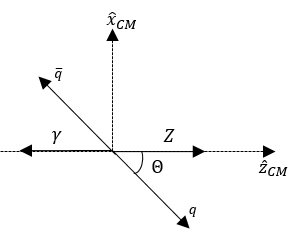
\includegraphics[width=0.3\textwidth]{fig/MVA/HZg_angle2.png}
		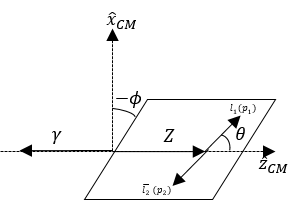
\includegraphics[width=0.3\textwidth]{fig/MVA/HZg_angle1.png}
	\end{center}
	\caption{Definitions of theoretical angles used for kinematic BDT training. The left diagram is in the Higgs boson center-of-mass frame, and the right diagram is in the $\PZ$ boson center-of-mass frame.}
	\label{fig:kinangles}
\end{figure}

\begin{figure}[tb]
	\begin{center}
		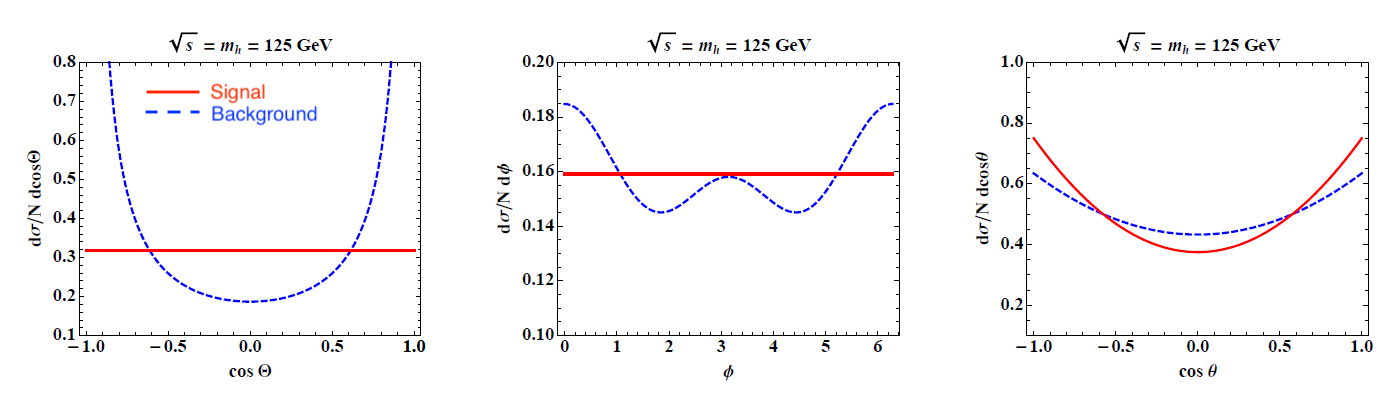
\includegraphics[width=0.9\textwidth]{fig/MVA/Zg_theorist.png}
		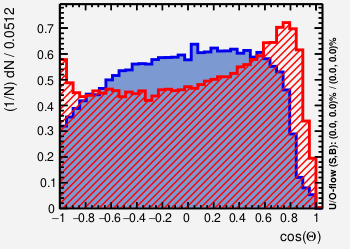
\includegraphics[width=0.3\textwidth]{fig/MVA/cosTheta_reco.png}
		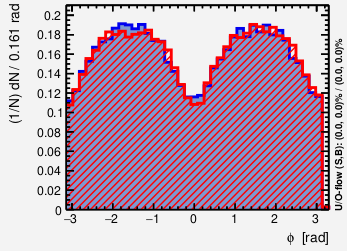
\includegraphics[width=0.3\textwidth]{fig/MVA/phi_reco.png}
		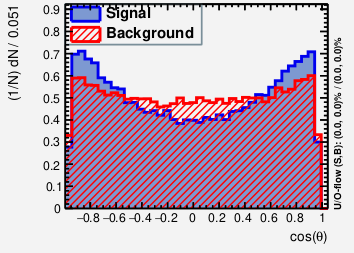
\includegraphics[width=0.3\textwidth]{fig/MVA/costheta_reco.png}
	\end{center}
	\caption[Top: Expected theoretical shapees for the angular features used for kinematic BDT training. Bottom: Reconstructed shapes for these quantities after the \hzg{} selection requirements have been applied. Please note that the red and blue color conventions are reversed for the top and bottom plots.]
	{Top: Expected theoretical shapes~\cite{HZg_angle1} for the angular features used for kinematic BDT training. Bottom: Reconstructed shapes for these quantities after the \hzg{} selection requirements have been applied. Please note that the red and blue color conventions are reversed for the top and bottom plots.} \label{fig:kin_GEN_angles}
\end{figure}

Several fundamental kinematic quantities of the final state particles are also used as training features. These include the pseudorapidity of each lepton, the $\Delta R$ between each lepton and the photon, and the $\pt/m$ of the $\lplm\gamma$ system. We note that the \pt values of each final state particle were also considered for training, but were found to have a negligible impact on discrimination power. This is likely because they are highly correlated with these other fundamental kinematic quantities, and thus, do not introduce much additional information to the BDT model. A comparison between signal and background shapes for these kinematic features is shown in Fig.~\ref{fig:kin_training_shapes}.

\begin{figure}[tb]
	\begin{center}
		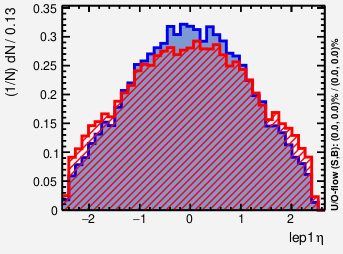
\includegraphics[width=0.3\textwidth]{fig/MVA/lepeta1_reco.png}
		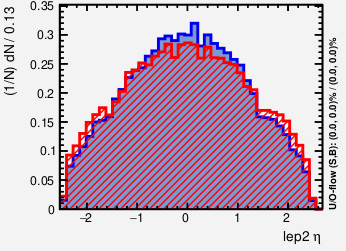
\includegraphics[width=0.3\textwidth]{fig/MVA/lepeta2_reco.png}
		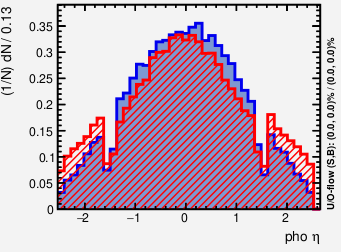
\includegraphics[width=0.3\textwidth]{fig/MVA/phoeta_reco.png}
		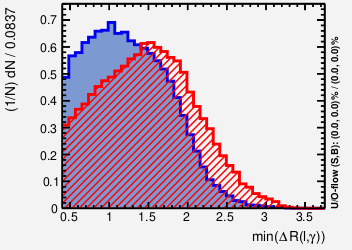
\includegraphics[width=0.3\textwidth]{fig/MVA/mindr_reco.png}
		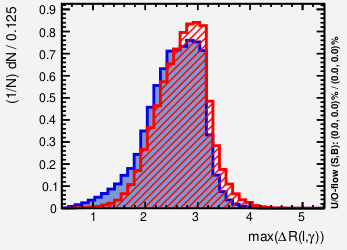
\includegraphics[width=0.3\textwidth]{fig/MVA/maxdr_reco.png}
		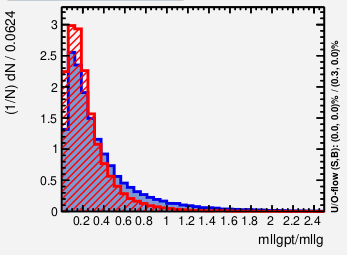
\includegraphics[width=0.3\textwidth]{fig/MVA/pt_over_m_reco.png}
	\end{center}
	\caption{Comparison of reconstructed signal and background shapes for several kinematic variables used for kinematic BDT training. The blue histograms represent the signal, while the red histograms represent the background.}
	\label{fig:kin_training_shapes}
\end{figure}

Finally, training features related to the quality of the final state photon are used. These include the corrected photon MVA ID score and the photon energy resolution. There are several motivations for these features. First, they are important for distinguishing \hzg{} signal events from the large $\PZ$+jets background, where a jet is misreconstructed as a photon. Second, they are inspired by the previous CMS \hzg{} searches, which used photon pseudorapidity and $R_{9}$ for categorization. In our current analysis, the photon $R_{9}$ was also considered as a training feature. However, it did not contribute any meaningful additional discriminating power. This is likely because the $R_9$ is already part of the corrected photon MVA ID. Figure~\ref{fig:kin_pho_features} shows the comparison between signal and background shapes for these features after the full set of \hzg{} selection requirements has been applied. Both features offer strong discrimination power, particularly the corrected photon MVA ID score. However, we note that this is partially by construction, since a very loose photon MVA ID cut was applied in order to preserve maximal information for the kinematic BDT training.

\begin{figure}[tb]
	\begin{center}
		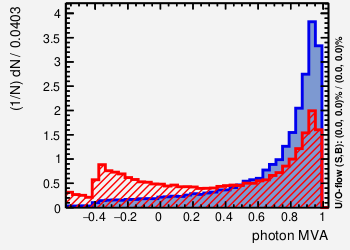
\includegraphics[width=0.35\textwidth]{fig/MVA/phomva_reco.png}
		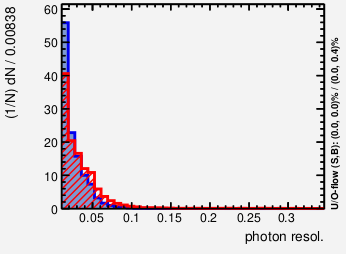
\includegraphics[width=0.35\textwidth]{fig/MVA/phores_reco.png}
	\end{center}
	\caption{Comparison of reconstructed signal and background shapes for the photon quality features used for kinematic BDT training. The blue histograms represent the signal, while the red histograms represent the background.}
	\label{fig:kin_pho_features}
\end{figure}

Since the kinematic BDT training is carried out using simulated events, it is necessary to check that the simulation accurately models the training feature distributions in data. 
A comparison of data to simulation, combining all years of data-taking in both the electron and muon channels, is shown in Fig.~\ref{fig:kin_vars1}. We observe good agreement between
data and simulation for all kinematic BDT training features. 

\begin{figure}[tb]
	\begin{center}
		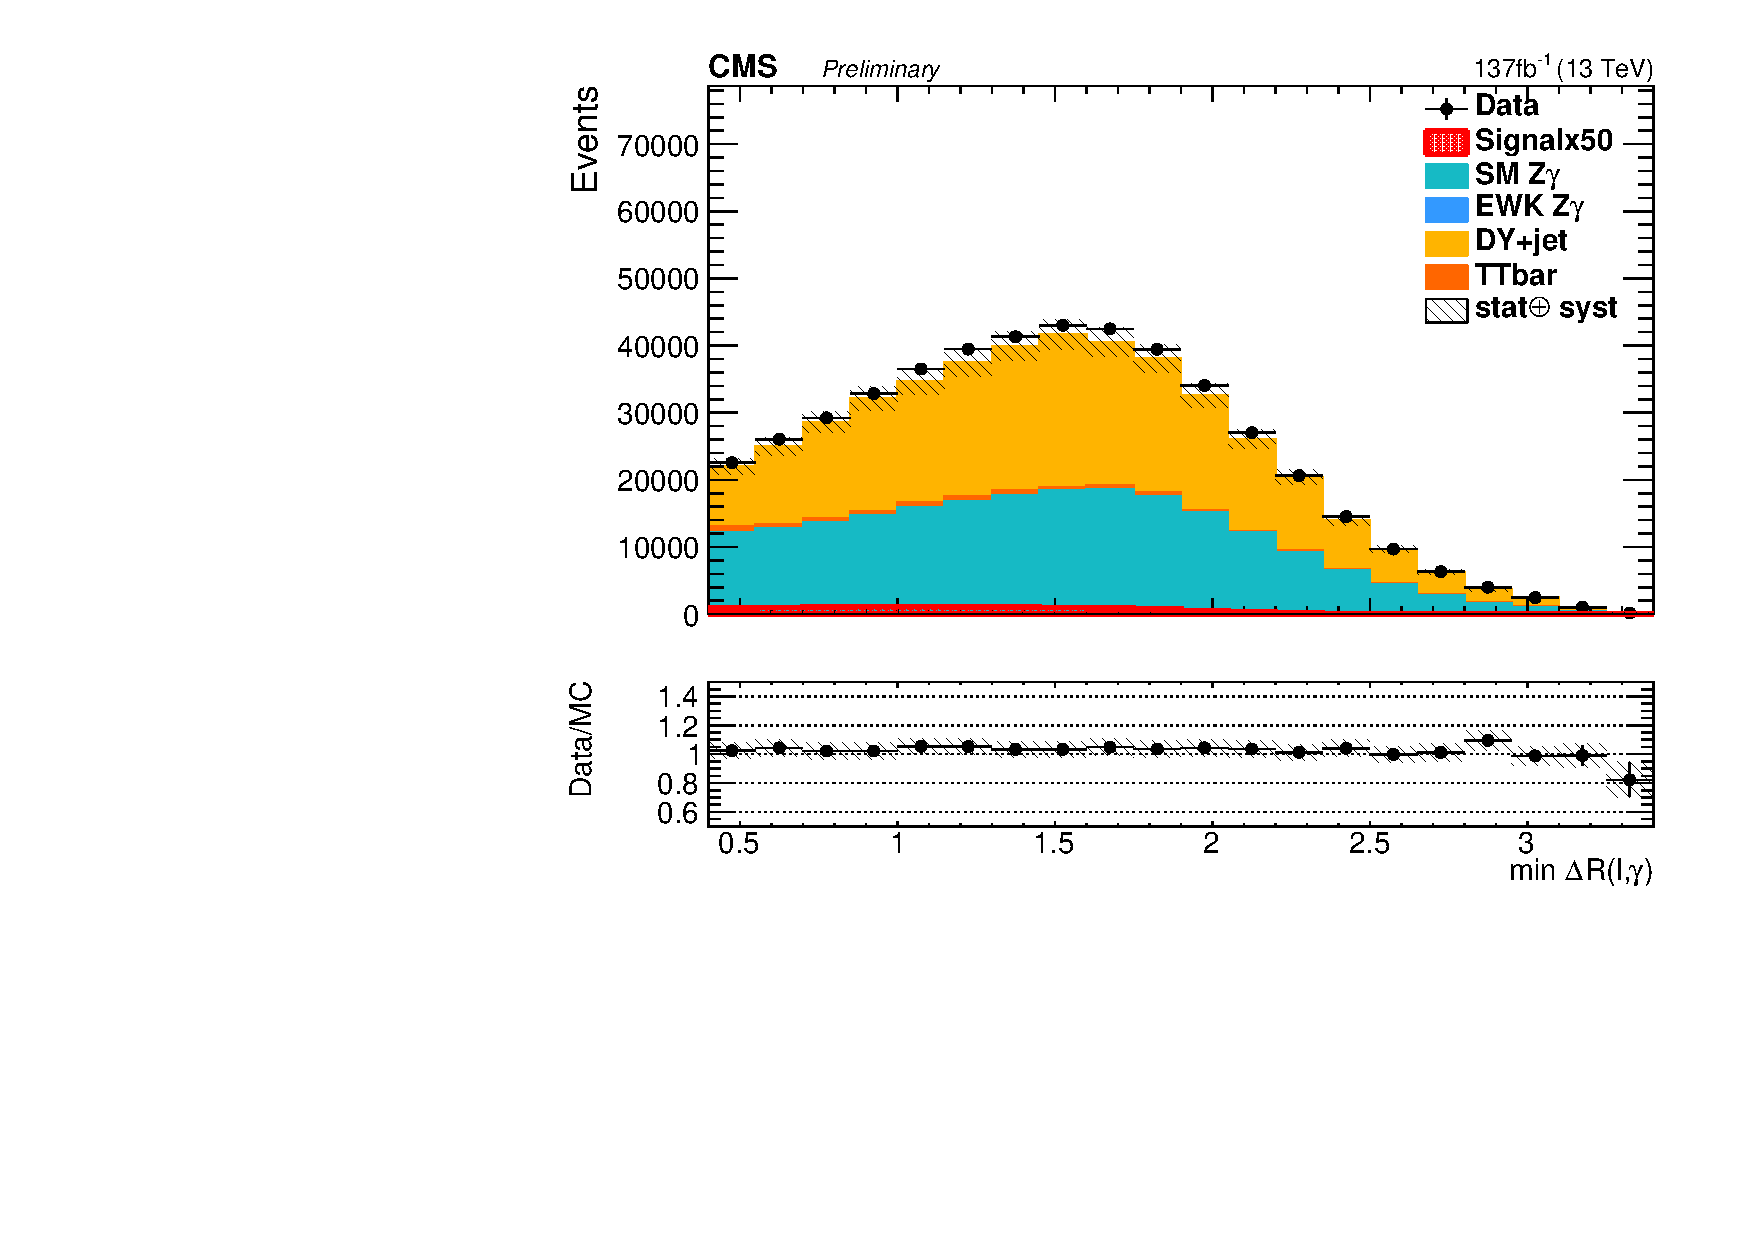
\includegraphics[width=0.32\textwidth]{fig/MVA/sc_all_kin_dRlg1_valid_ptwei_cat0.pdf}
		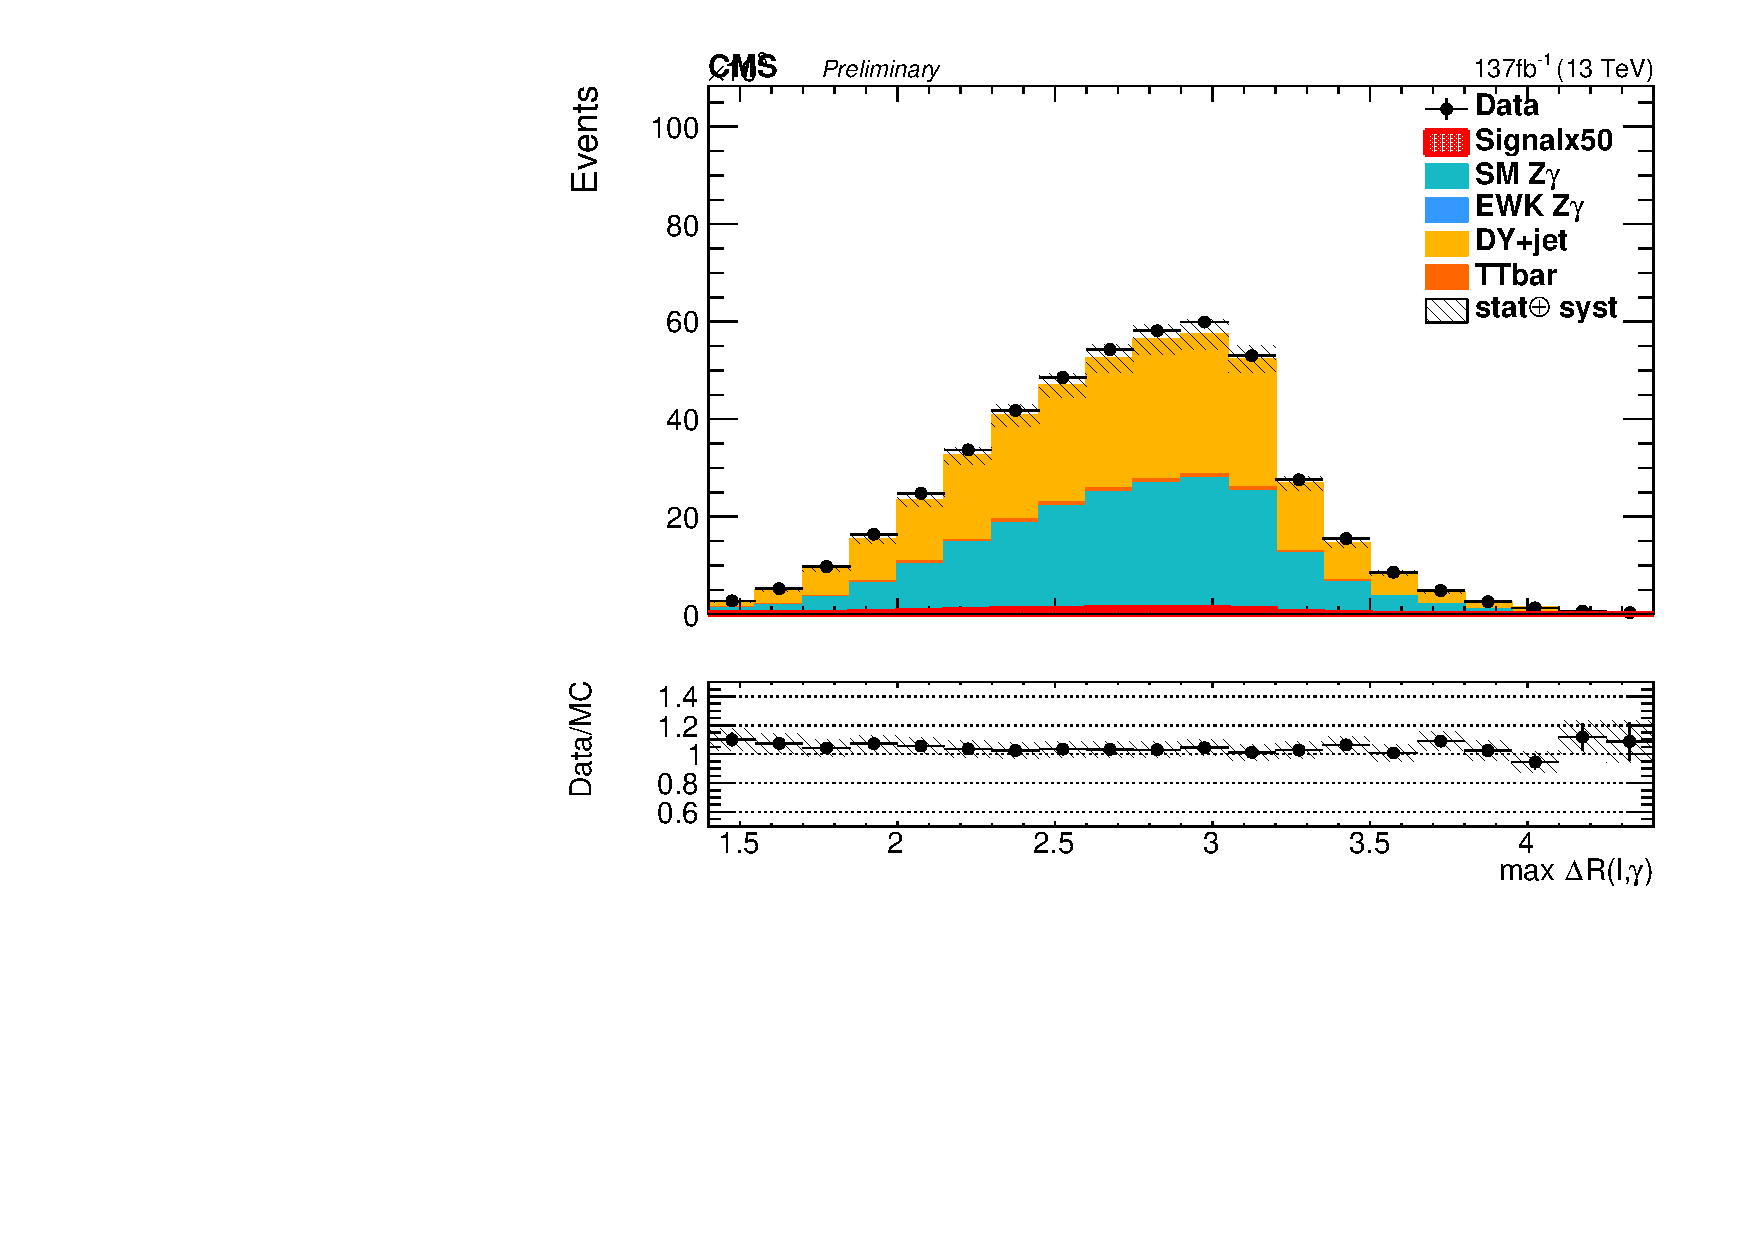
\includegraphics[width=0.32\textwidth]{fig/MVA/sc_all_kin_dRlg2_valid_ptwei_cat0.pdf}
		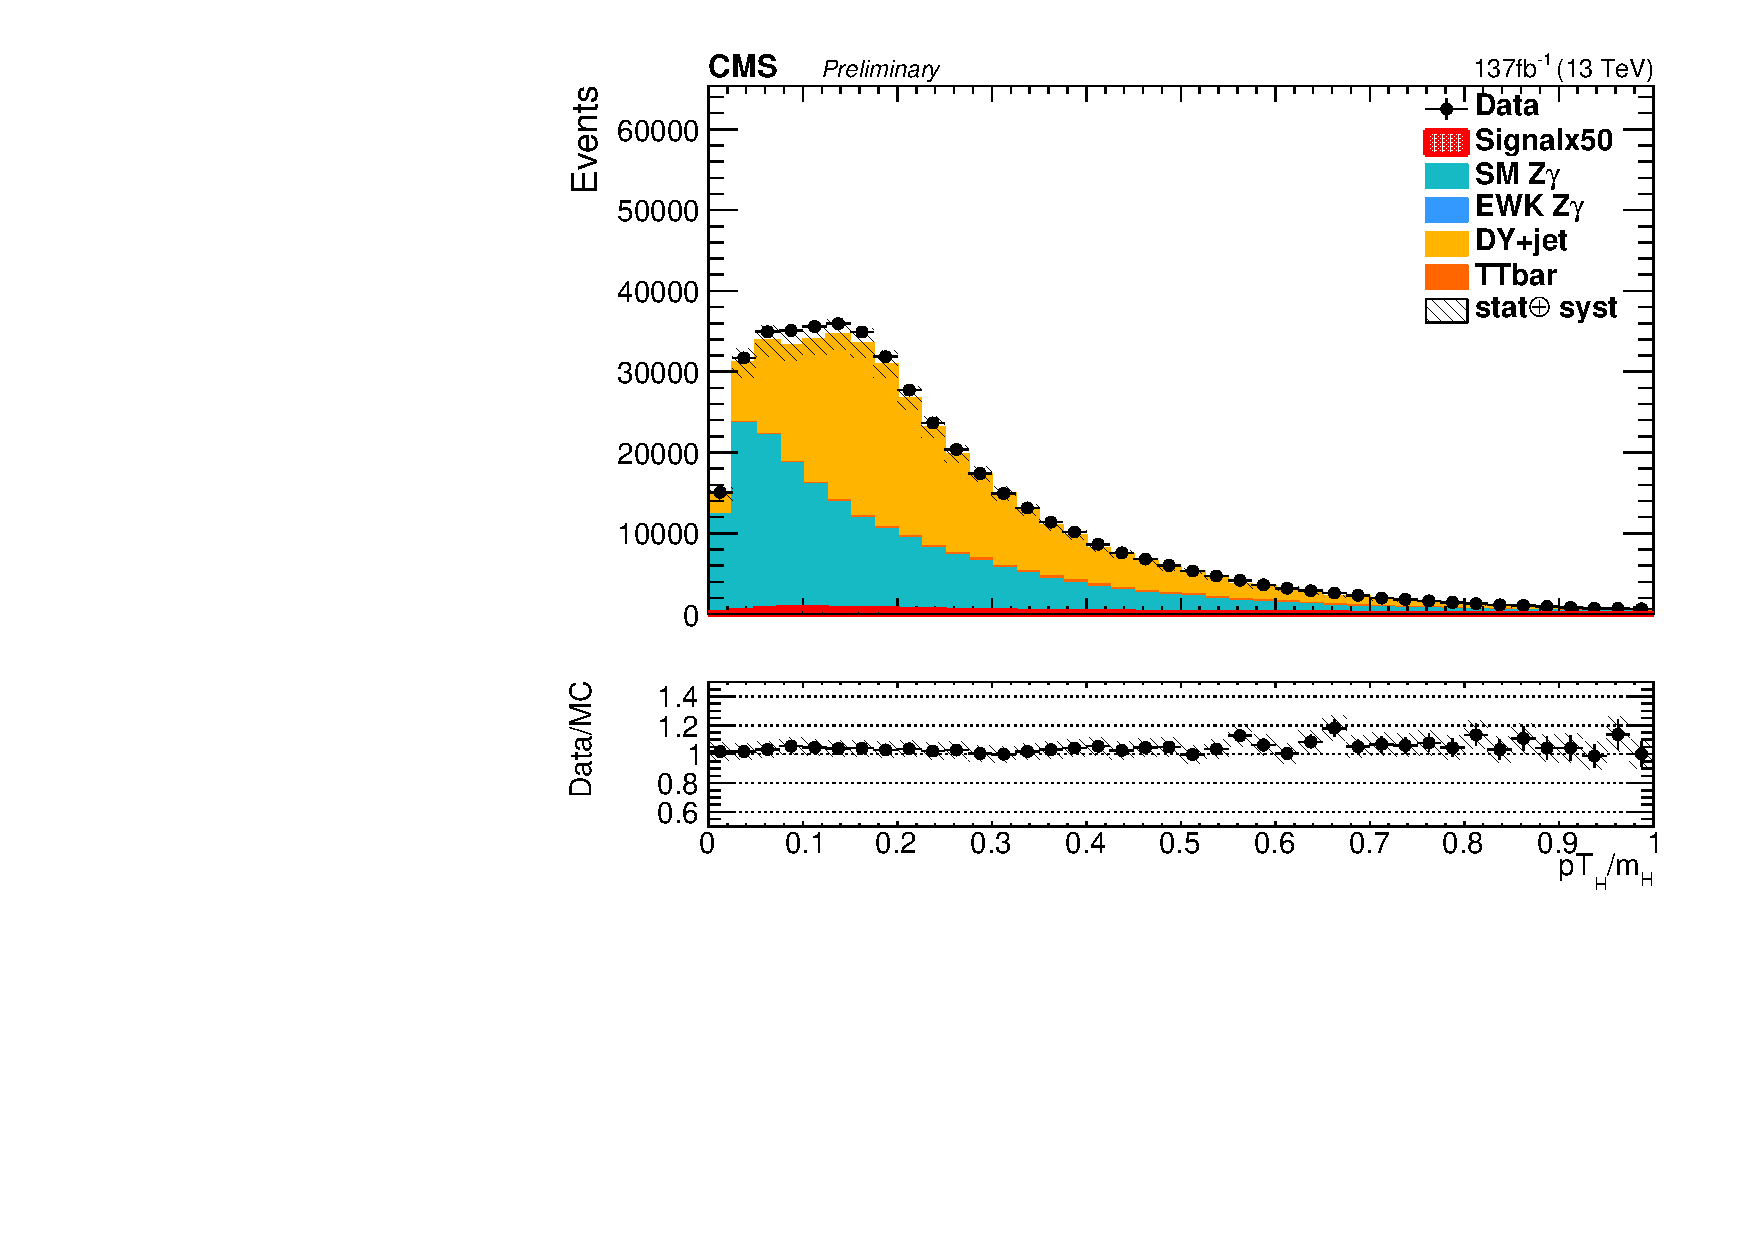
\includegraphics[width=0.32\textwidth]{fig/MVA/sc_all_kin_mllgmllgpt_valid_ptwei_cat0.pdf}\\
		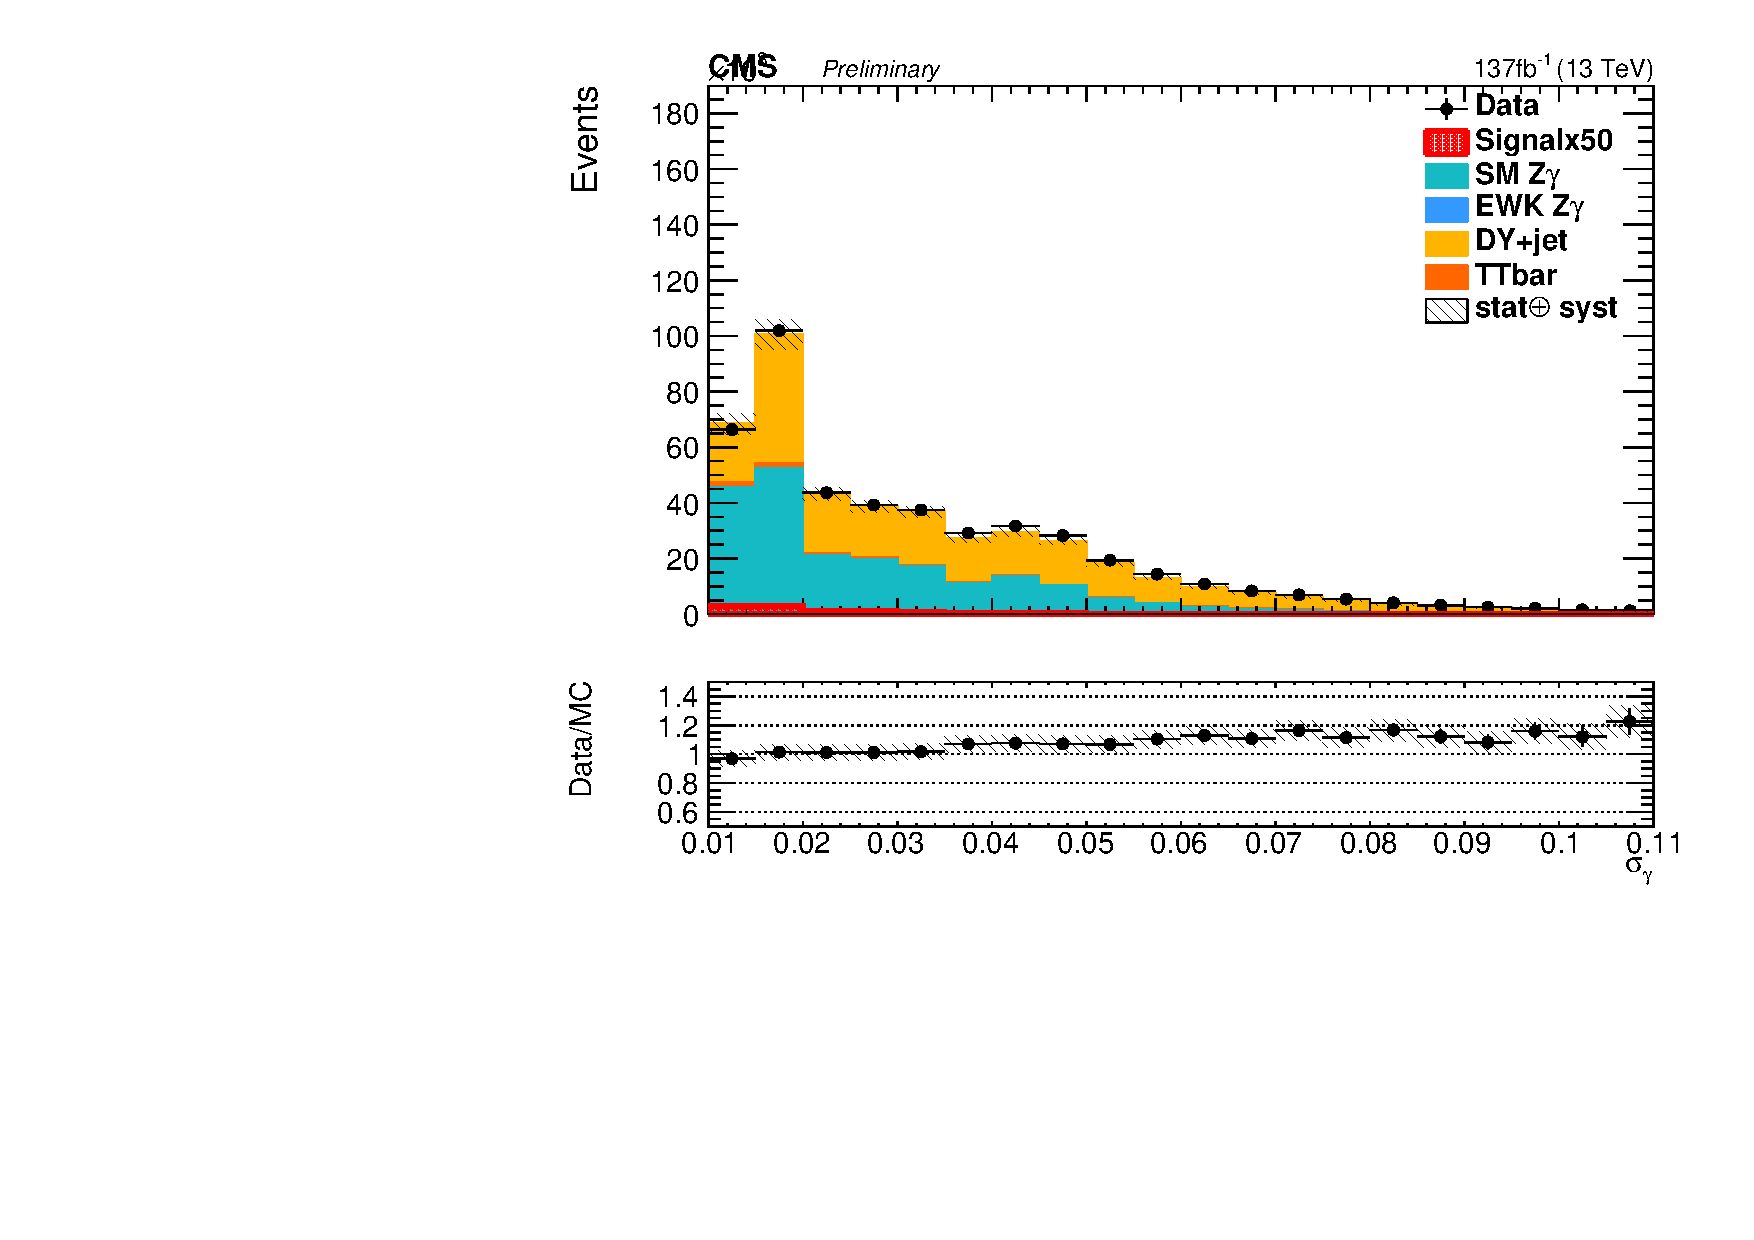
\includegraphics[width=0.32\textwidth]{fig/MVA/sc_all_kin_phores_valid_ptwei_cat0.pdf}
		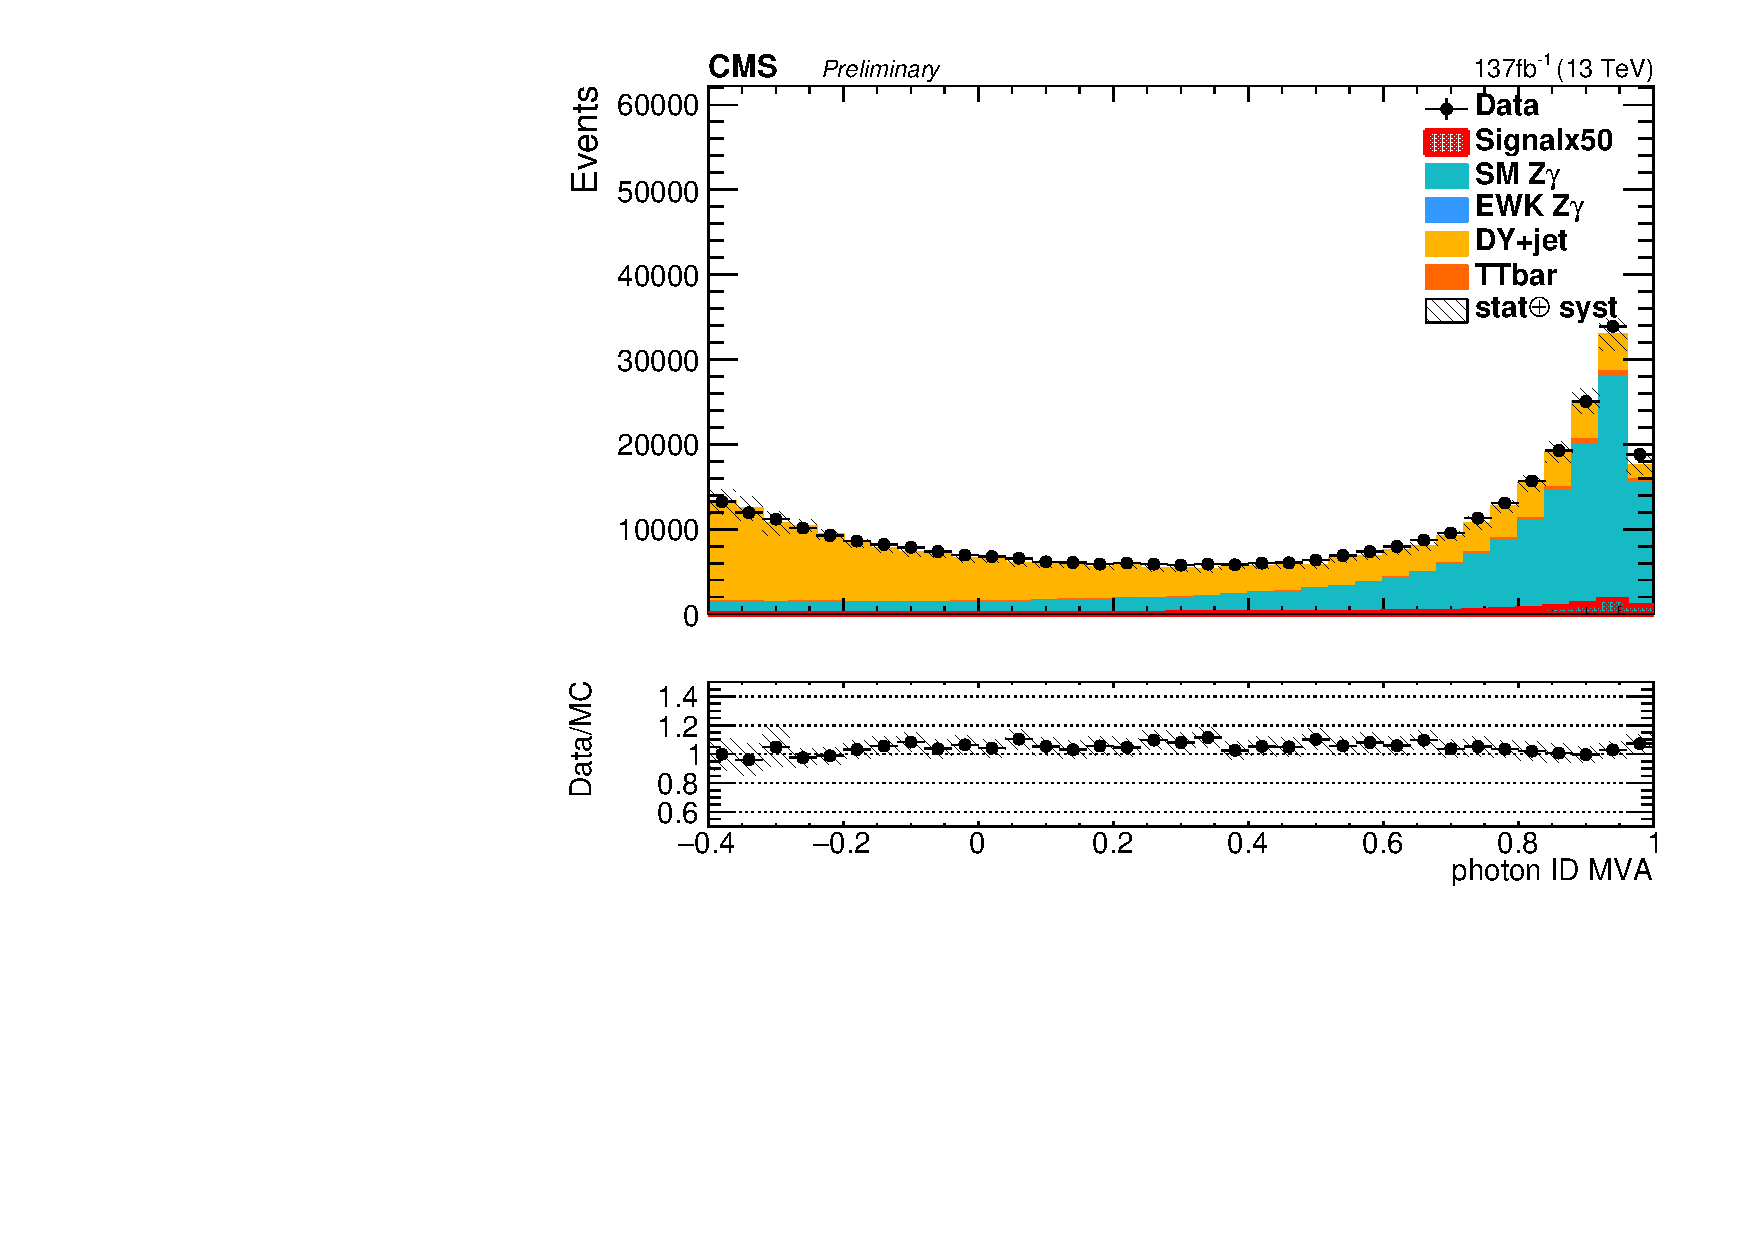
\includegraphics[width=0.32\textwidth]{fig/MVA/sc_all_kin_phomva_valid_ptwei_EB_cat0.pdf}
		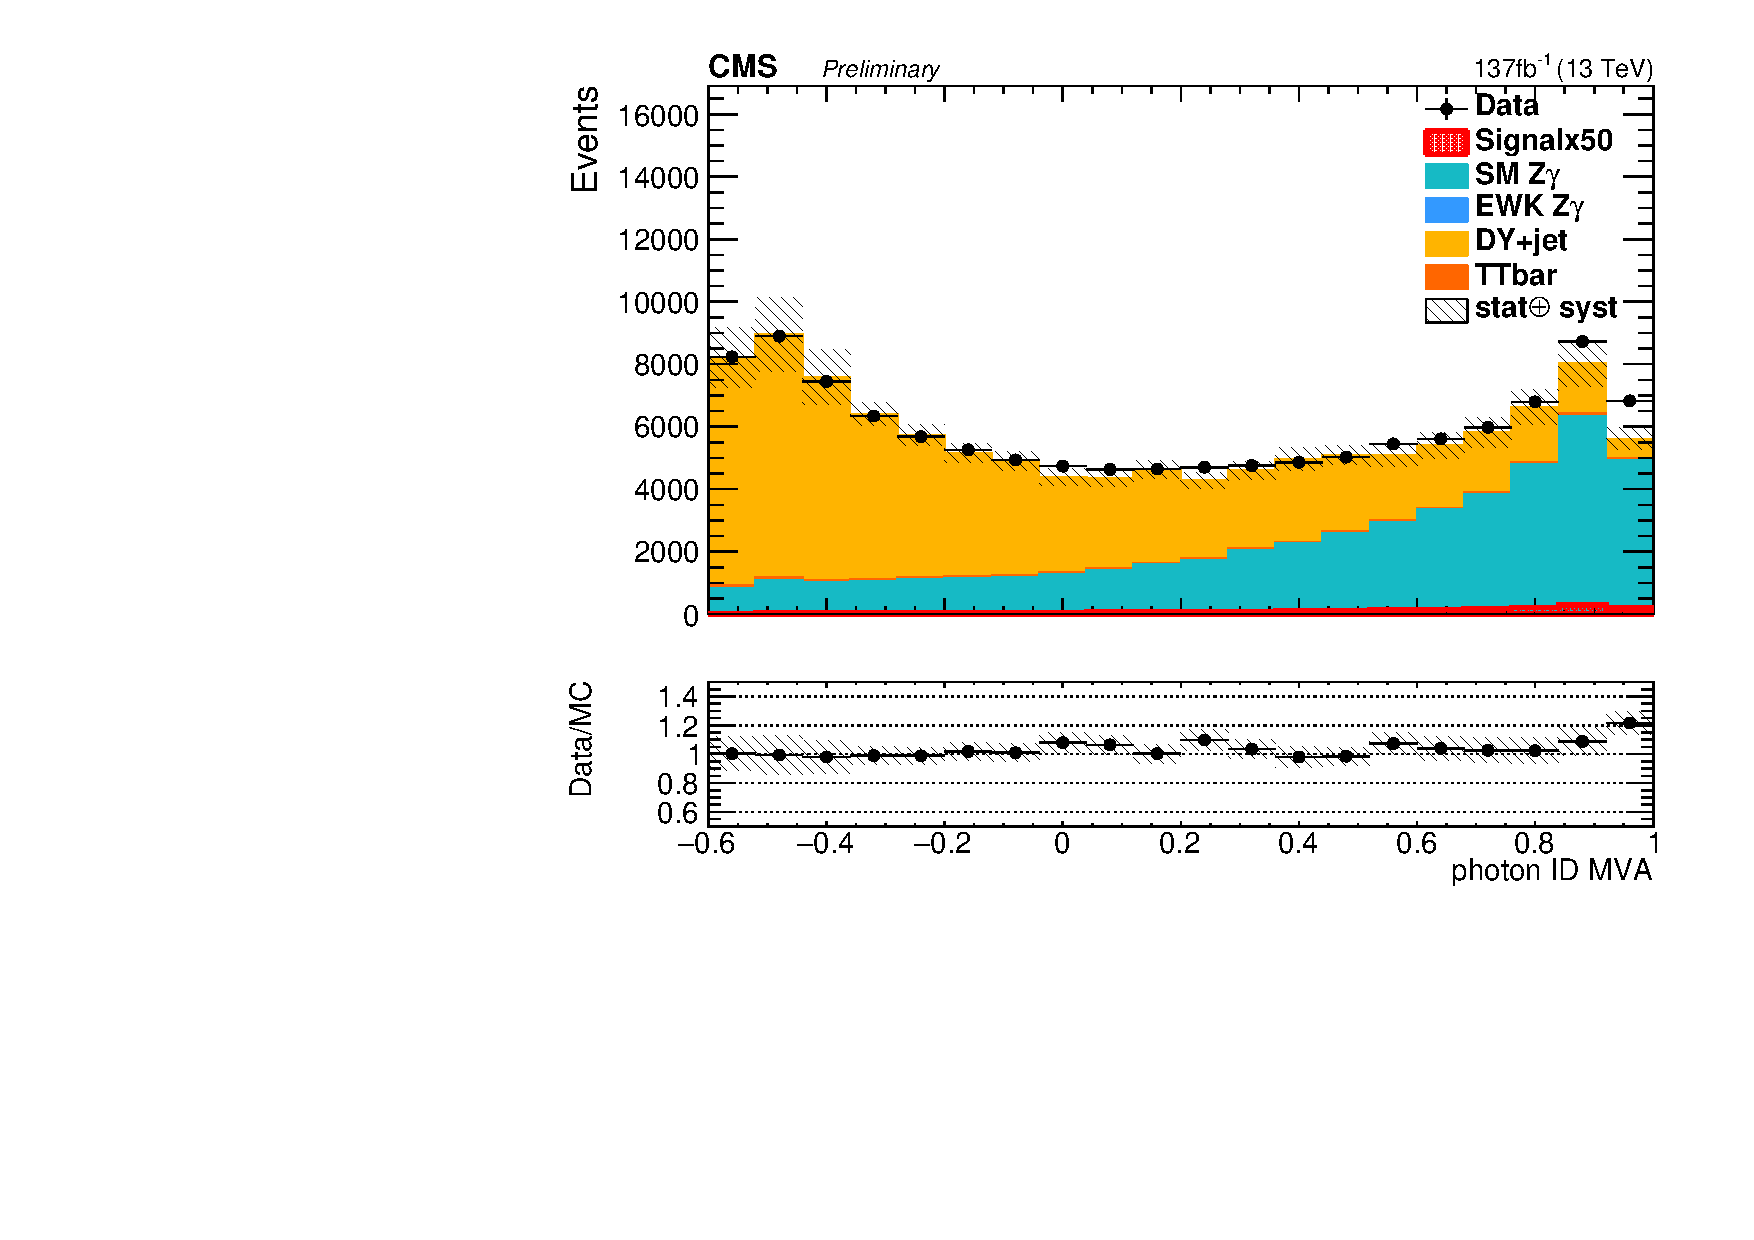
\includegraphics[width=0.32\textwidth]{fig/MVA/sc_all_kin_phomva_valid_ptwei_EE_cat0.pdf}\\
		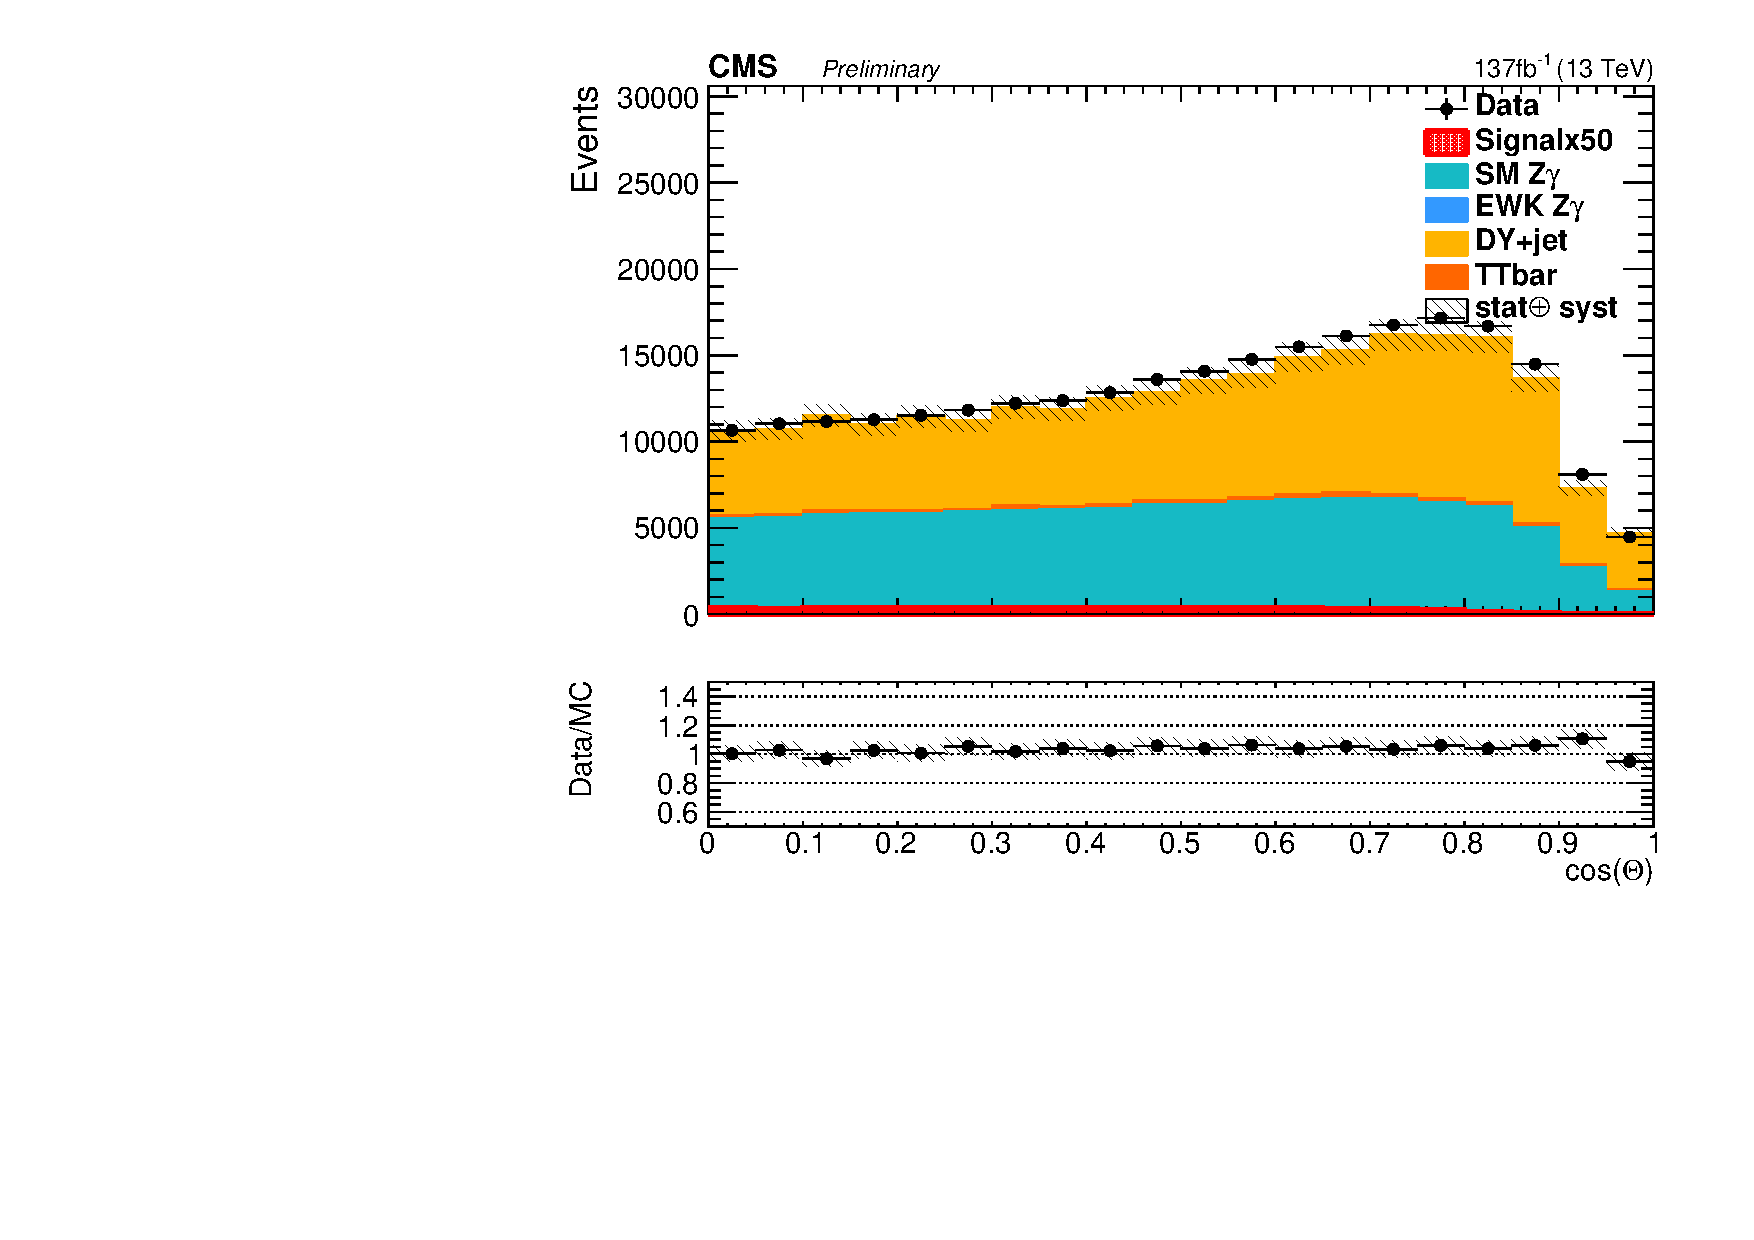
\includegraphics[width=0.32\textwidth]{fig/MVA/sc_all_kin_coscaptheta_valid_ptwei_cat0.pdf}
		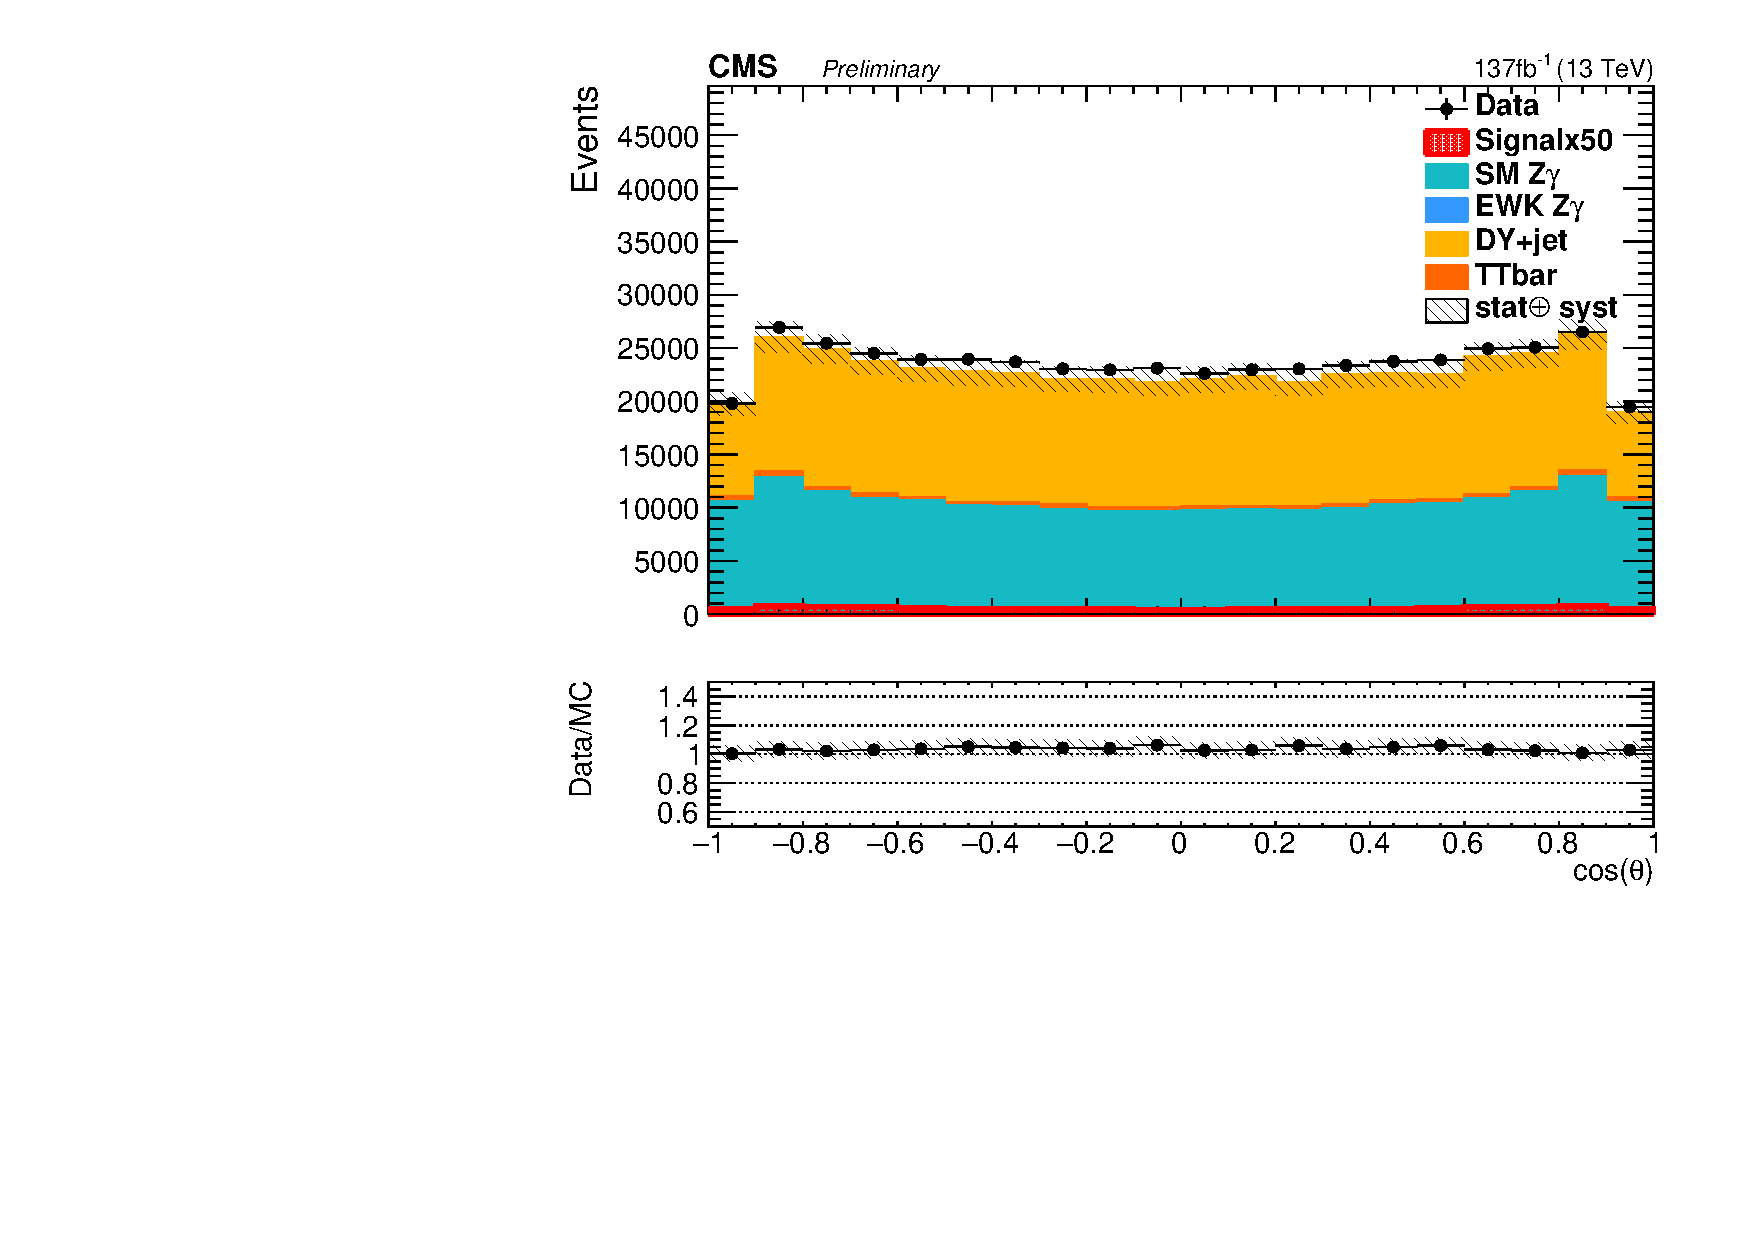
\includegraphics[width=0.32\textwidth]{fig/MVA/sc_all_kin_costheta_valid_ptwei_cat0.pdf}
		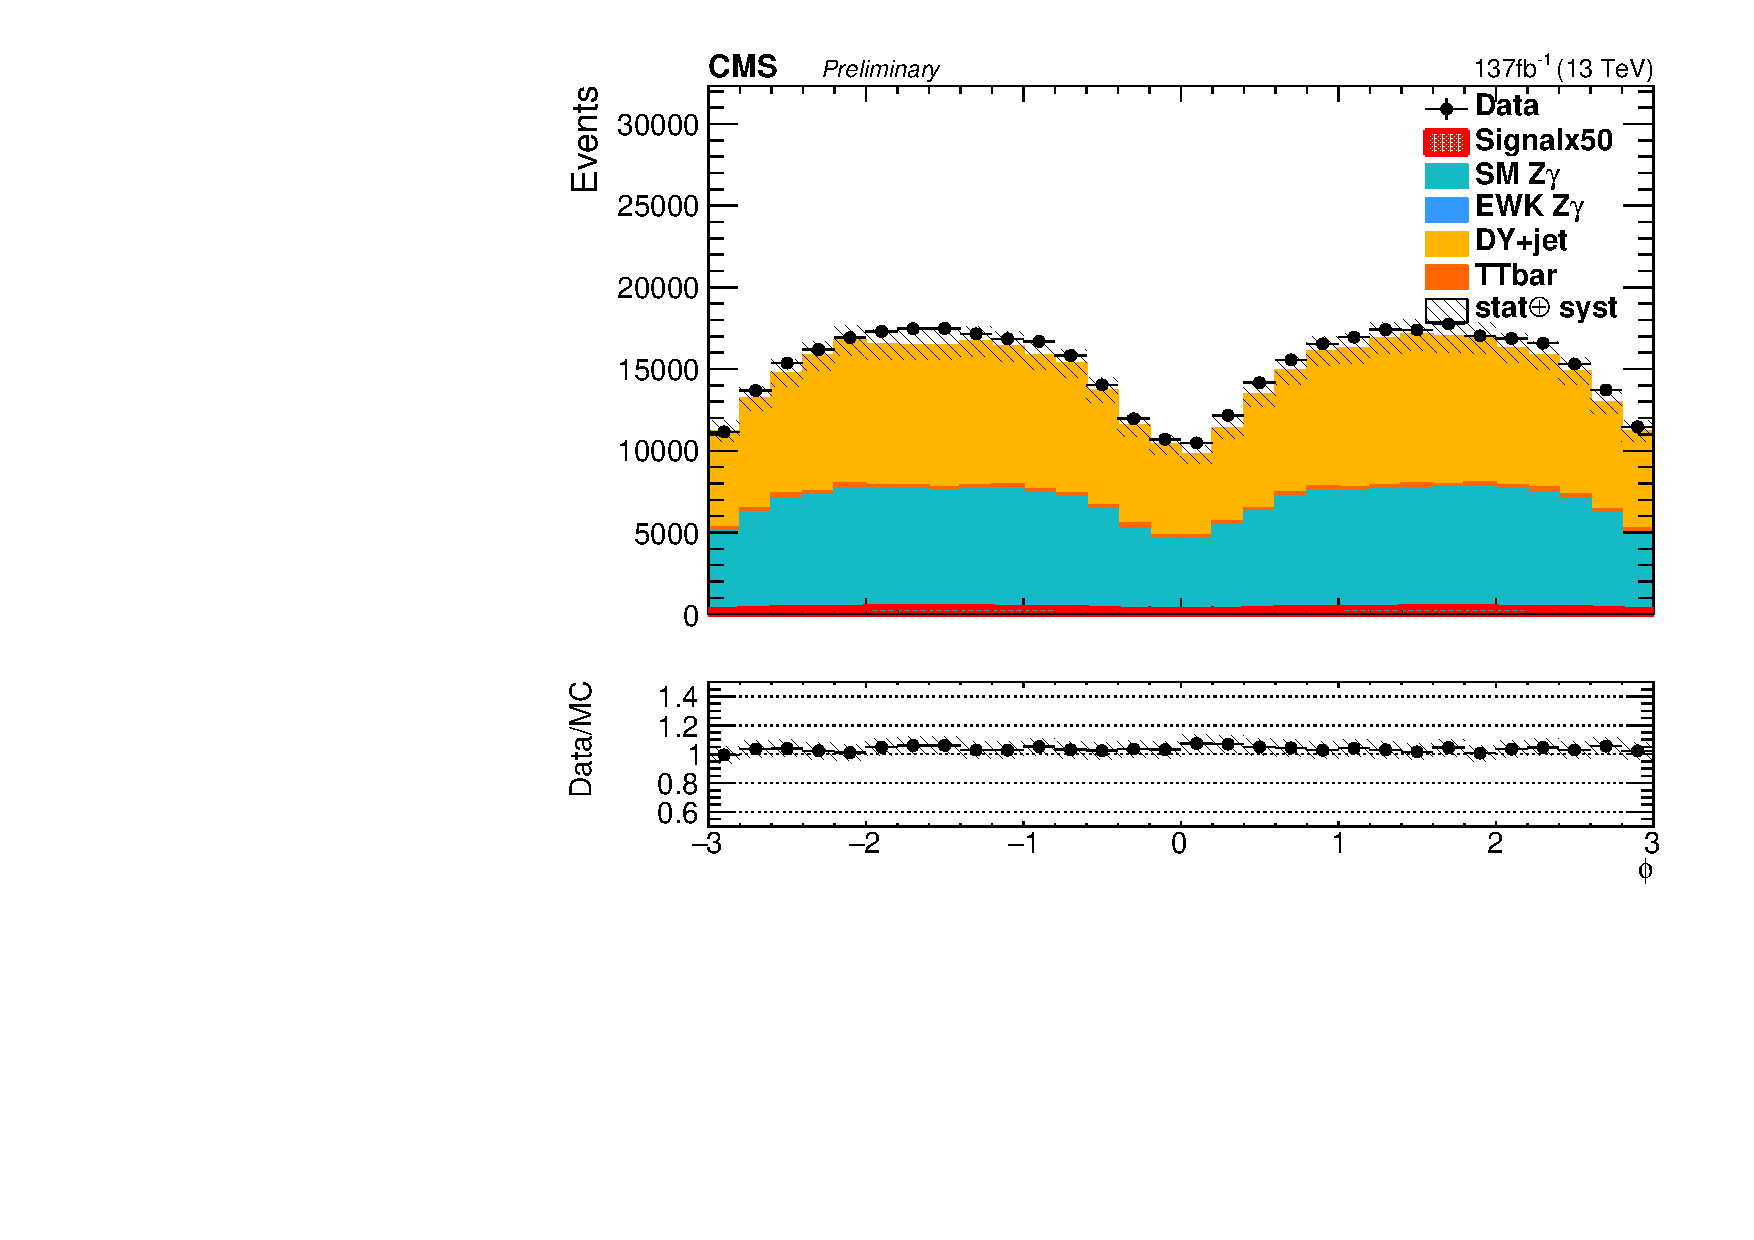
\includegraphics[width=0.32\textwidth]{fig/MVA/sc_all_kin_phi_valid_ptwei_cat0.pdf}\\
		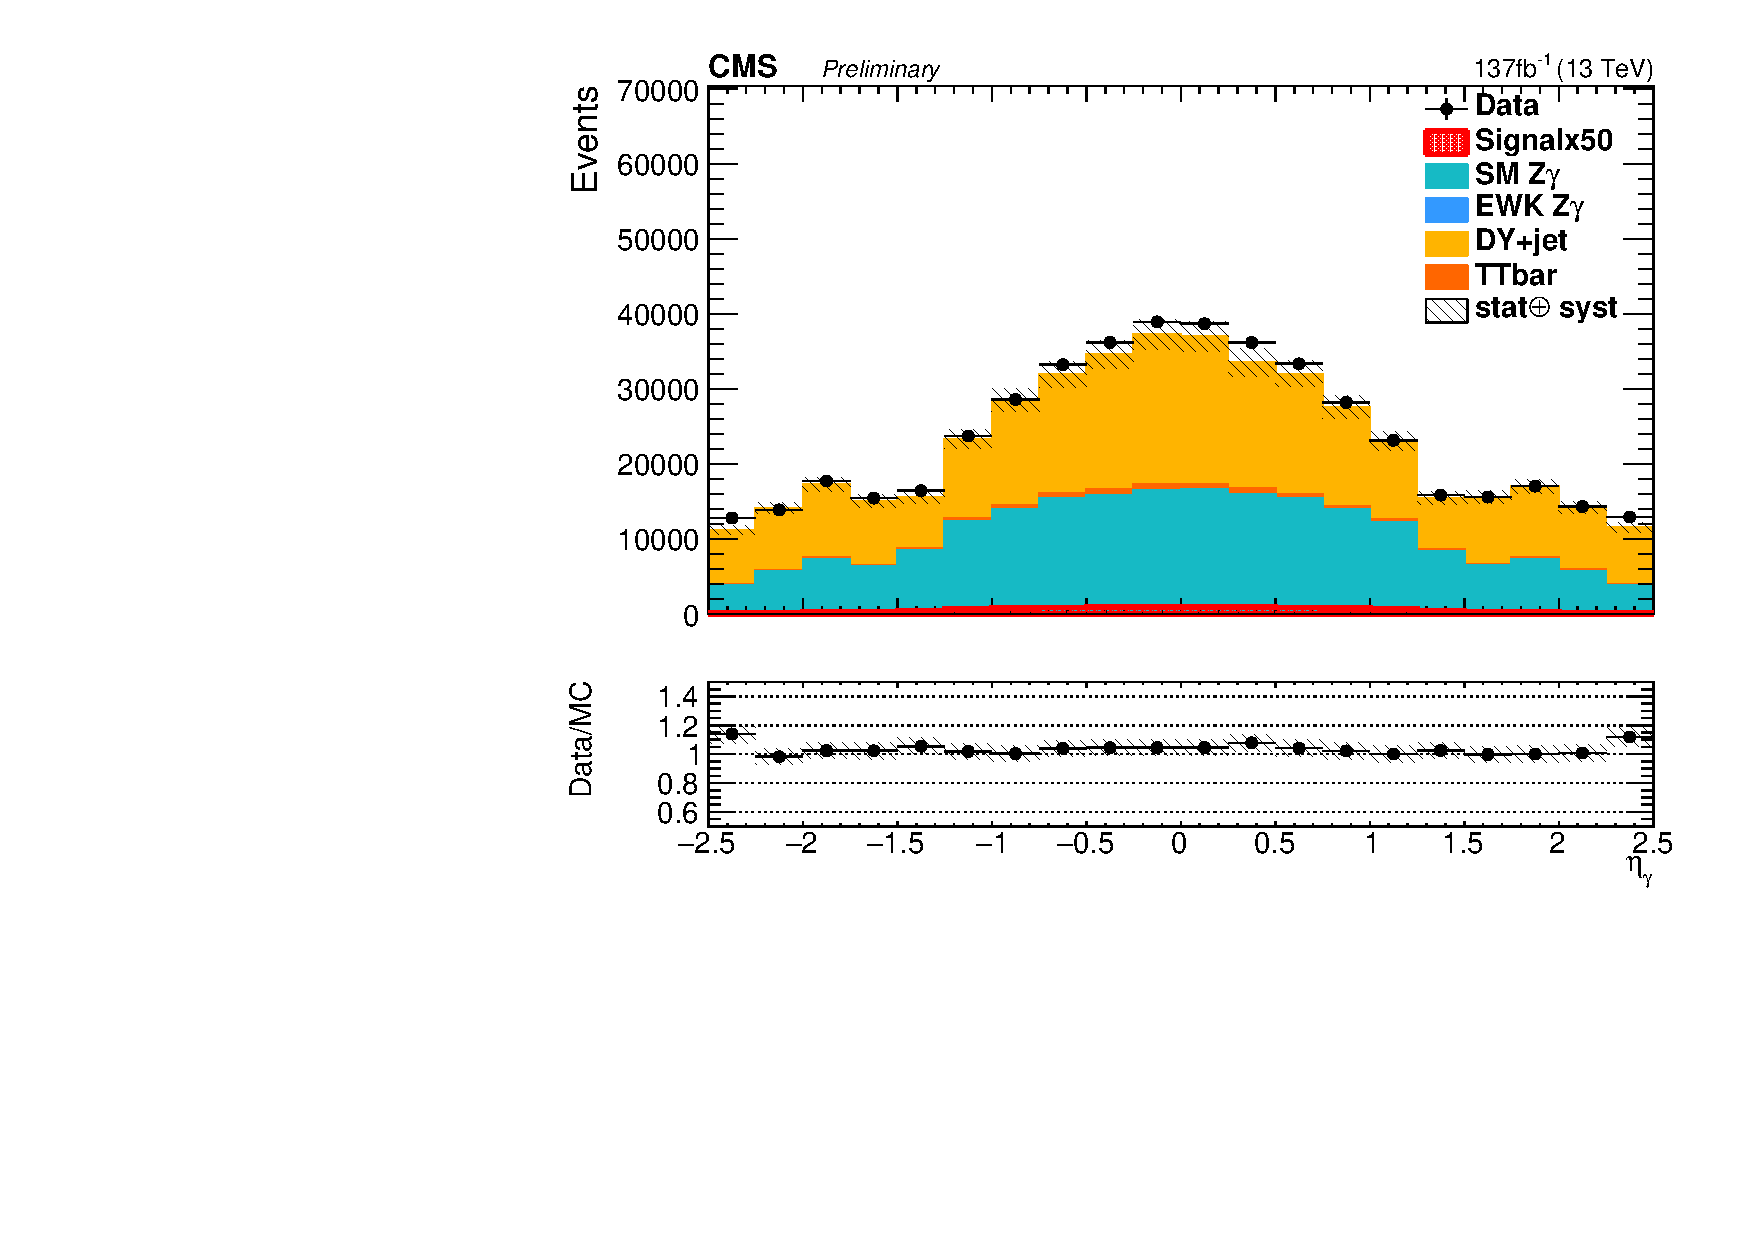
\includegraphics[width=0.32\textwidth]{fig/MVA/sc_all_kin_phoeta_valid_ptwei_cat0.pdf}
		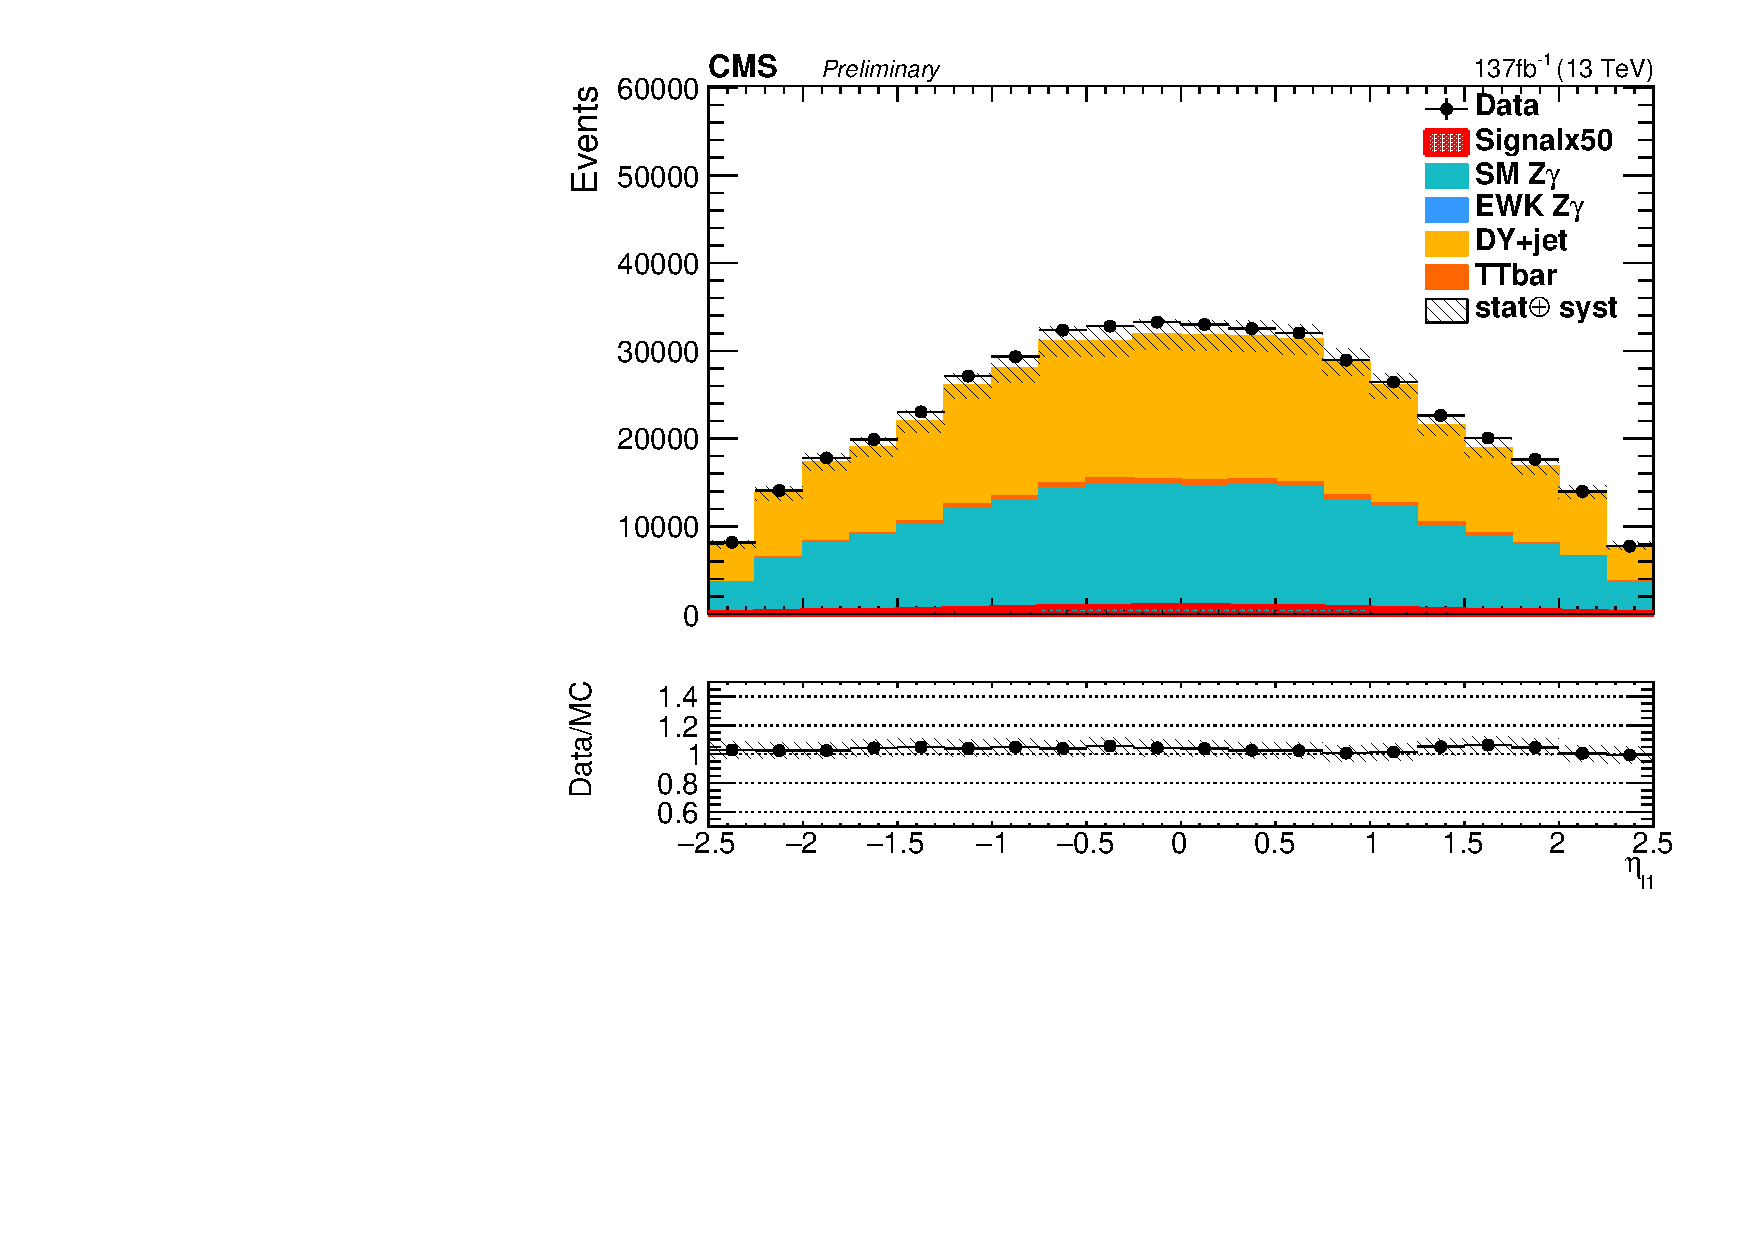
\includegraphics[width=0.32\textwidth]{fig/MVA/sc_all_kin_lepeta1_valid_ptwei_cat0.pdf}
		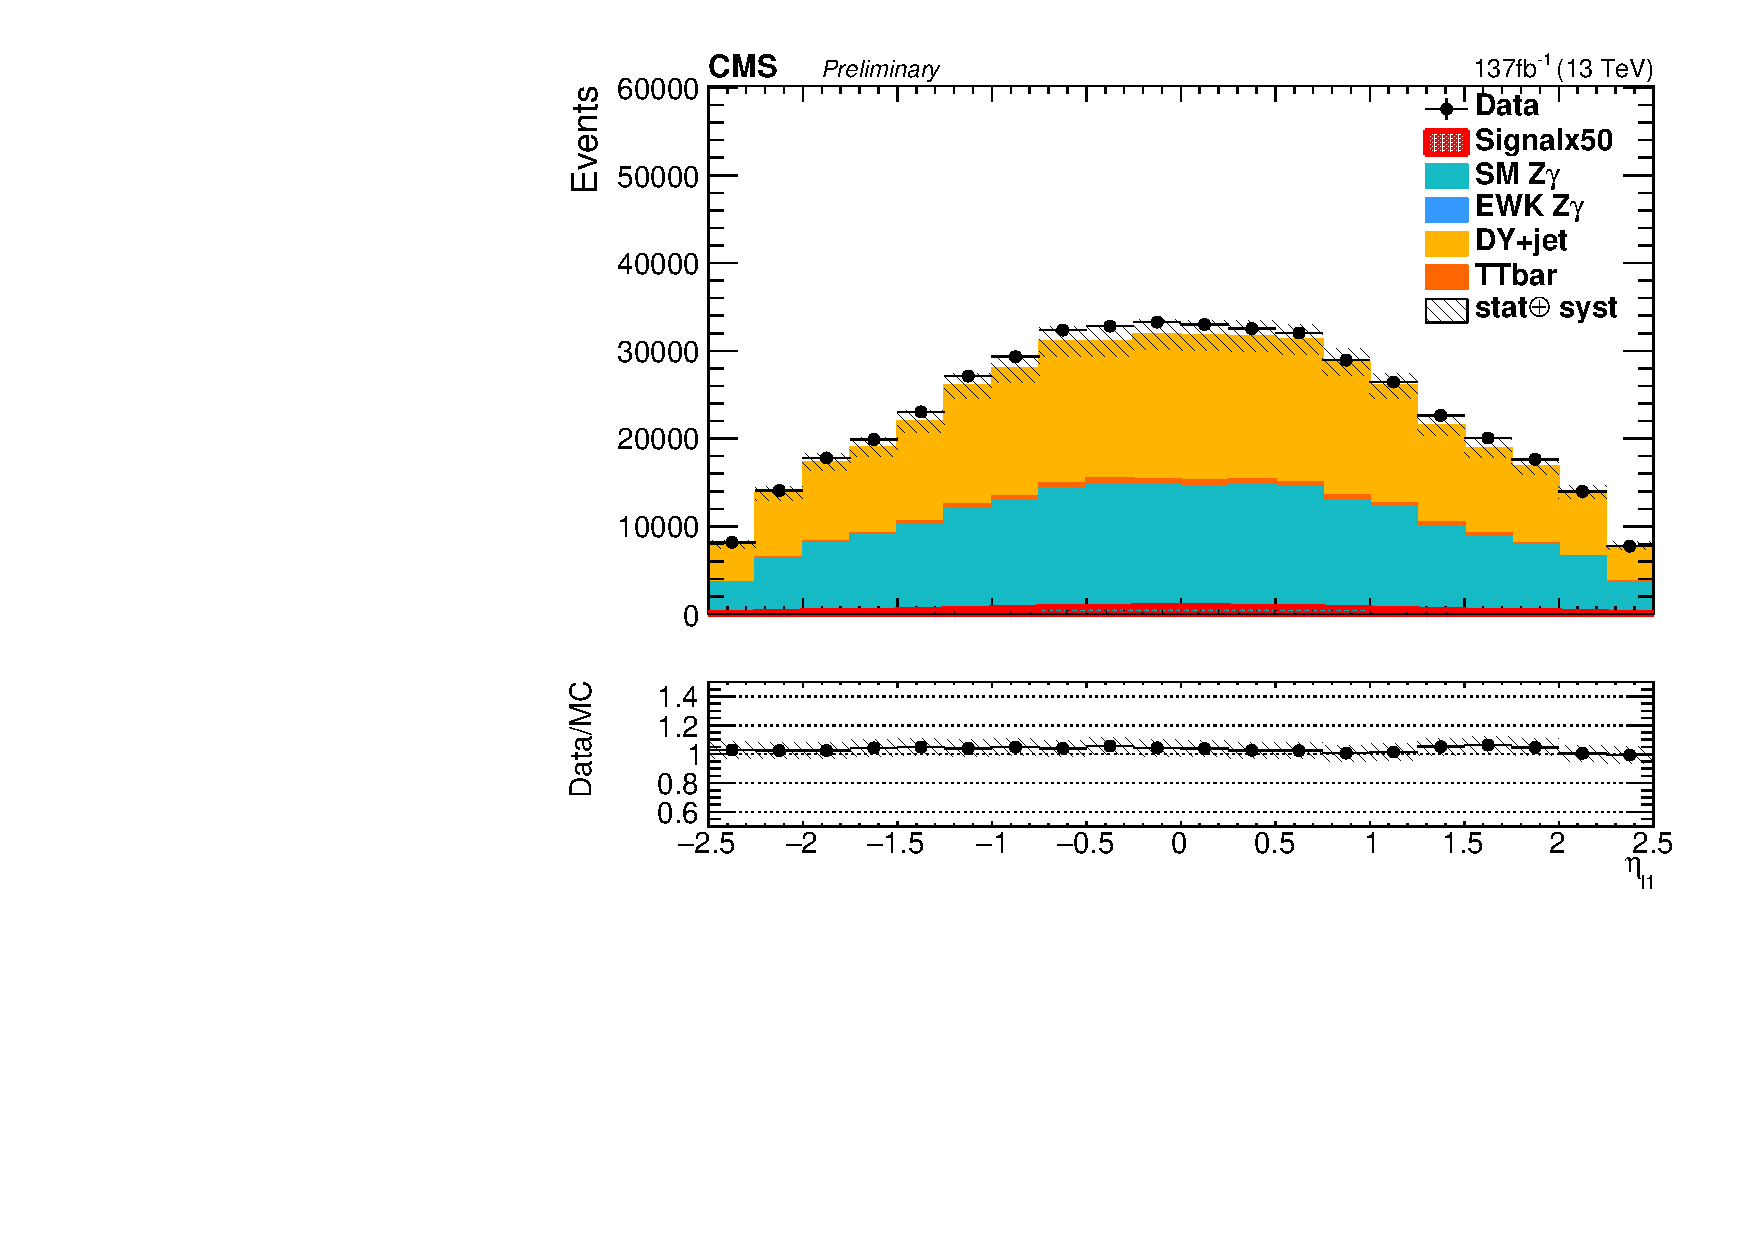
\includegraphics[width=0.32\textwidth]{fig/MVA/sc_all_kin_lepeta1_valid_ptwei_cat0.pdf}\\
		\end{center}
	\caption{Comparison of data and simulation for the kinematic BDT training features. The plotted distributions include data and simulated samples from the combination of the three 
	data-taking years in both the electron and muon channels.}
	\label{fig:kin_vars1}
\end{figure}

\subsection{Training Results}
The output kinematic BDT shapes for signal and background are shown in Fig.~\ref{fig:kin_overtrain}. No overtraining is observed, 
as evidenced by the similarity between training and test distributions. The importance of each training feature for the discrimination power of
the final kinematic BDT discriminant is given in Table~\ref{tab:kin_importance}. We see that the corrected photon MVA score is the most discriminating 
feature, since it distinguishes real photons from misreconstructed jets. The variable $\pt^{\lplm\gamma}/m_{\lplm\gamma}$ also contributes good discimination power, and 
effectively replaces the need for a boosted Higgs category, as was used in the CMS 2016 search. 

\begin{figure}[tb]
	\begin{center}
		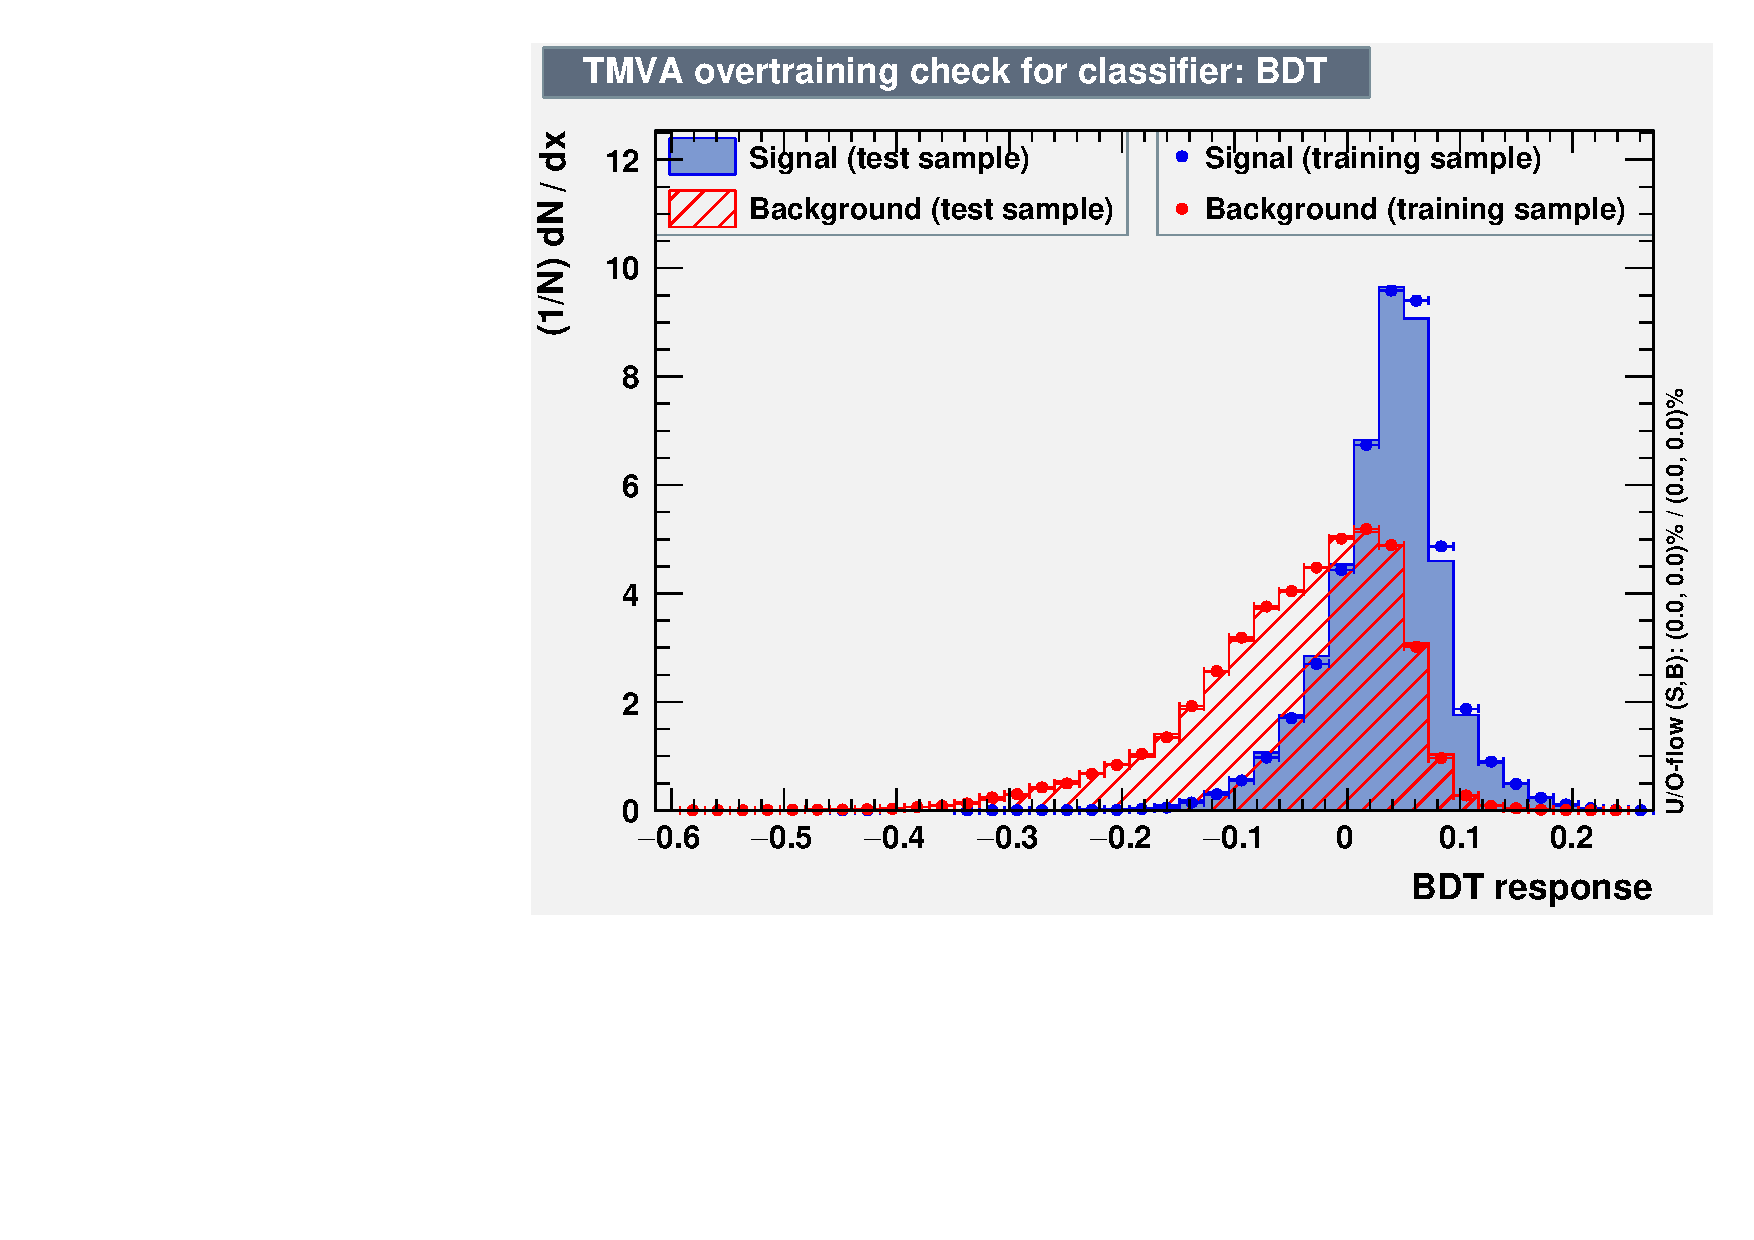
\includegraphics[width=0.65\textwidth]{fig/MVA/kin_overtrain_BDT.pdf}
	\end{center}
	\caption{Shapes of the kinematic BDT distributions for signal and background for both training and test sets. No BDT overtraining is observed.}\label{fig:kin_overtrain}
\end{figure}

\begin{table}[tb]
	\centering
	\begin{tabular}{|c c|}
		\hline
		               Variable                & Variable Importance (\%) \\ \hline
				corrected photon MVA score 				& 12.8     \\
		       	min($\Delta R(\ell,\gamma)$) 				& 12.0      \\
		      	$\pt^{\lplm\gamma}/m_{\lplm\gamma}$ 	 	& 10.2 	  \\
		        	$\cos{\Theta}$	 					& 10.0		 \\
		     	$\frac{\sigma_{\gamma}}{E_\gamma}$     			& 9.1		 \\
		        	$\cos{\theta}$ 						& 8.2      \\
		          max($\Delta R(\ell,\gamma))$ 	              		& 8.1	\\
		 	   	$\eta_{\ell 2}$      					& 8.1      \\
		      	$\eta_{\ell 1}$        					& 7.9 \\
		      	$\eta_\gamma$ 				 		& 7.2      \\
		          $\phi$                    				& 6.2  \\\hline

	\end{tabular}
 \caption{Importance of the kinematic BDT training features.}
\label{tab:kin_importance}
\end{table}

\section{Vector Boson Fusion Boosted Decision Tree}
The VBF BDT is used to discriminate signal events arising via the VBF Higgs production mechanism from other sources of signal and background events. 
The training and evaluation of the VBF BDT is carried out on events that have two jets selected according to the requirements in 
Chapter~\ref{sec:selection}. Signal events for training are taken from the simulated VBF \hzg{} samples, while ggH \hzg{}, $\PZ\gamma$, $\PZ$+jets, and 
$\ttbar$ events are considered background. Due to their very small contribution, $\mathrm{V}\PH$ and $\ttbar\PH$ \hzg{} events are neglected. Only about 65\% 
of the selected jets from the VBF signal correspond to the true VBF jets in which we are interested. Because of this, we perform an additional matching 
procedure for these jets. In order for a VBF signal event to be used in the training, both reconstructed jets must be matched 
to generator-level partons, which must, in turn, be matched to the generator-level \pt values of the true VBF partons. 
Only half of the simulated events satisfying this requirement are used for the training procedure, with the remainder used for category optimization
and signal $m_{\lplm\gamma}$ shape modeling. Events from all three data-taking years in both the muon and electron channels are combined for training, weighted by the respective cross sections 
and by the recorded integrated luminosity of each data-taking year.

\subsection{Training Features}
The training features used for the VBF BDT include quantities that distinguish events with the VBF topology from other types of events, as well as quantities that 
distinguish signal from background based on kinematics. Since the categorization strategy treats dijet events separately from other types of events, including these 
kinematic variables is not redundant with the kinematic BDT described above. The two variables used for kinematic separation of signal and background for the VBF BDT are 
the kinematic BDT score and the variable $p_{\mathrm{T}}^{t}$, defined in Chapter~\ref{sec:analysis_overview}. Because the kinematics of the two leptons and photon are 
similar for VBF signal events and other signal production mechanisms, the previously trained kinematic BDT is expected to yield good discrimation power between VBF signal and backgrounds. 
By introducing the variable $p_{\mathrm{T}}^{t}$, we add another feature sensitive to boost of the Higgs boson. This takes advantage of the recoil of the Higgs boson against the jets, and along 
with the variable $\pt^{\lplm\gamma}/m_{\lplm\gamma}$ in the kinematic BDT, replaces the need for a boosted category. Signal and background shapes for the kinematic BDT score and $p_{\mathrm{T}}^{t}$ are shown in Fig.~\ref{fig:kin_bdt_ptt}, where background refers to the full training background, including ggH \hzg{} events.

\begin{figure}[tb]
	\begin{center}
		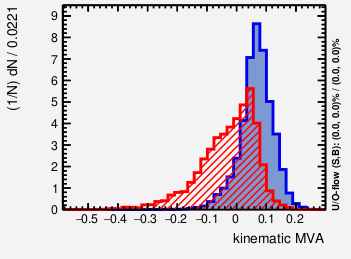
\includegraphics[width=0.35\textwidth]{fig/MVA/kin_bdt_vbf_training.png}
		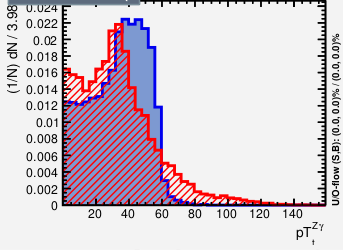
\includegraphics[width=0.35\textwidth]{fig/MVA/ptt_vbf_training.png}
	\end{center}
	\caption{Comparison of signal and background shapes for the kinematic features used for VBF BDT training. The blue histograms represent the VBF signal, while the red histograms represent the training background, including ggH \hzg{} events.}
	\label{fig:kin_bdt_ptt}
\end{figure}

We also include training features that aim to distinguish VBF events from non-VBF events, using information about the jets. These include 
  (i) the difference in 
  pseudorapidity between the two jets;
  (ii)  the difference in azimuthal angle
  between the  two jets; 
   (iii) the
  photon Zeppenfeld variable~\cite{Rainwater:1996ud} ($\eta_{\gamma} -
  (\eta_{\mathrm{j_1}}+\eta_{\mathrm{j_2}})/2$), where 
  $\eta_{\gamma} ,\eta_{\mathrm{j1}}$ and $\eta_\mathrm{{j2}}$ are the pseudorapidities of the
  photon, leading jet, and subleading jet, respectively; 
	(iv) the ratio between the $\pt$ of the $\PZ\gamma{\mathrm{j_1}}{\mathrm{j_2}}$ system and the corresponding scalar sum of momenta 
		($\abs{\sum_{Z\gamma\mathrm{j_1}\mathrm{j_2}}{\vec{p}_{\mathrm{T}}}} / \sum_{Z\gamma\mathrm{j_1}\mathrm{j_2}}p_\mathrm{T}$);
   (v) the difference in azimuthal angle
  between the dijet system and the $\PZ\gamma$ system;
  (vi) the $\pt$ of each jet; and (vii) the $\DR$ separation between each jet and the photon. Other training features were also 
  tried, including the individual pseudorapidities of the jets and the Zeppenfeld variable for the $\PZ\gamma$ system. However, 
  these features were not included, as they offered negligible improvement for the final trained model. Signal and background 
  shape comparisons for the above variables are shown in Fig.~\ref{fig:vbf_bdt_features}.

\begin{figure}[tb]
	\begin{center}
		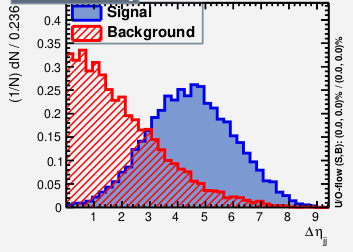
\includegraphics[width=0.3\textwidth]{fig/MVA/deta_jj_vbf.png}
		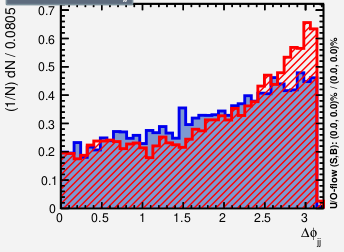
\includegraphics[width=0.3\textwidth]{fig/MVA/dphi_jj_vbf.png}
		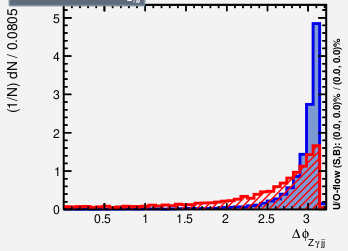
\includegraphics[width=0.3\textwidth]{fig/MVA/dphi_zgjj_vbf.png}
		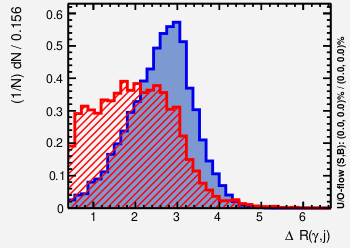
\includegraphics[width=0.3\textwidth]{fig/MVA/dr_gj_vbf.png}
		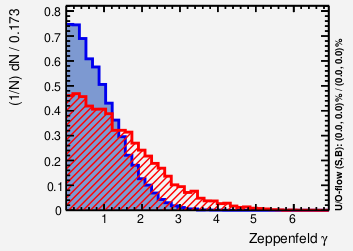
\includegraphics[width=0.3\textwidth]{fig/MVA/zepp_vbf.png}
		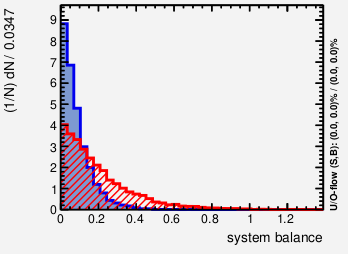
\includegraphics[width=0.3\textwidth]{fig/MVA/ptbal_vbf.png}
		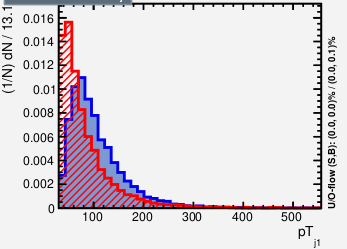
\includegraphics[width=0.3\textwidth]{fig/MVA/ptj1_vbf.png}
		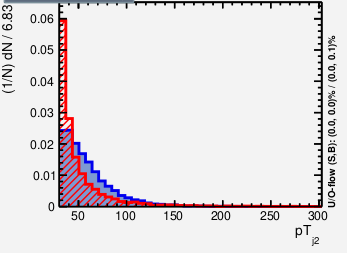
\includegraphics[width=0.3\textwidth]{fig/MVA/ptj2_vbf.png}
	\end{center}
	\caption{Comparison of signal and background shapes for several variables used for VBF BDT training. The blue histograms represent the VBF signal, while the red histograms represent the training background, including ggH \hzg{} events.}
	\label{fig:vbf_bdt_features}
\end{figure}

Since the VBF BDT training is carried out using simulated events, it is necessary to check that the simulation accurately models the training feature distributions in data. 
A comparison of data to simulation, combining all years of data-taking in both the electron and muon channels, is shown in Fig.~\ref{fig:VBF_valid}. We observe good agreement between
data and simulation for all VBF BDT training features. 

\begin{figure}[tb]
	\begin{center}
		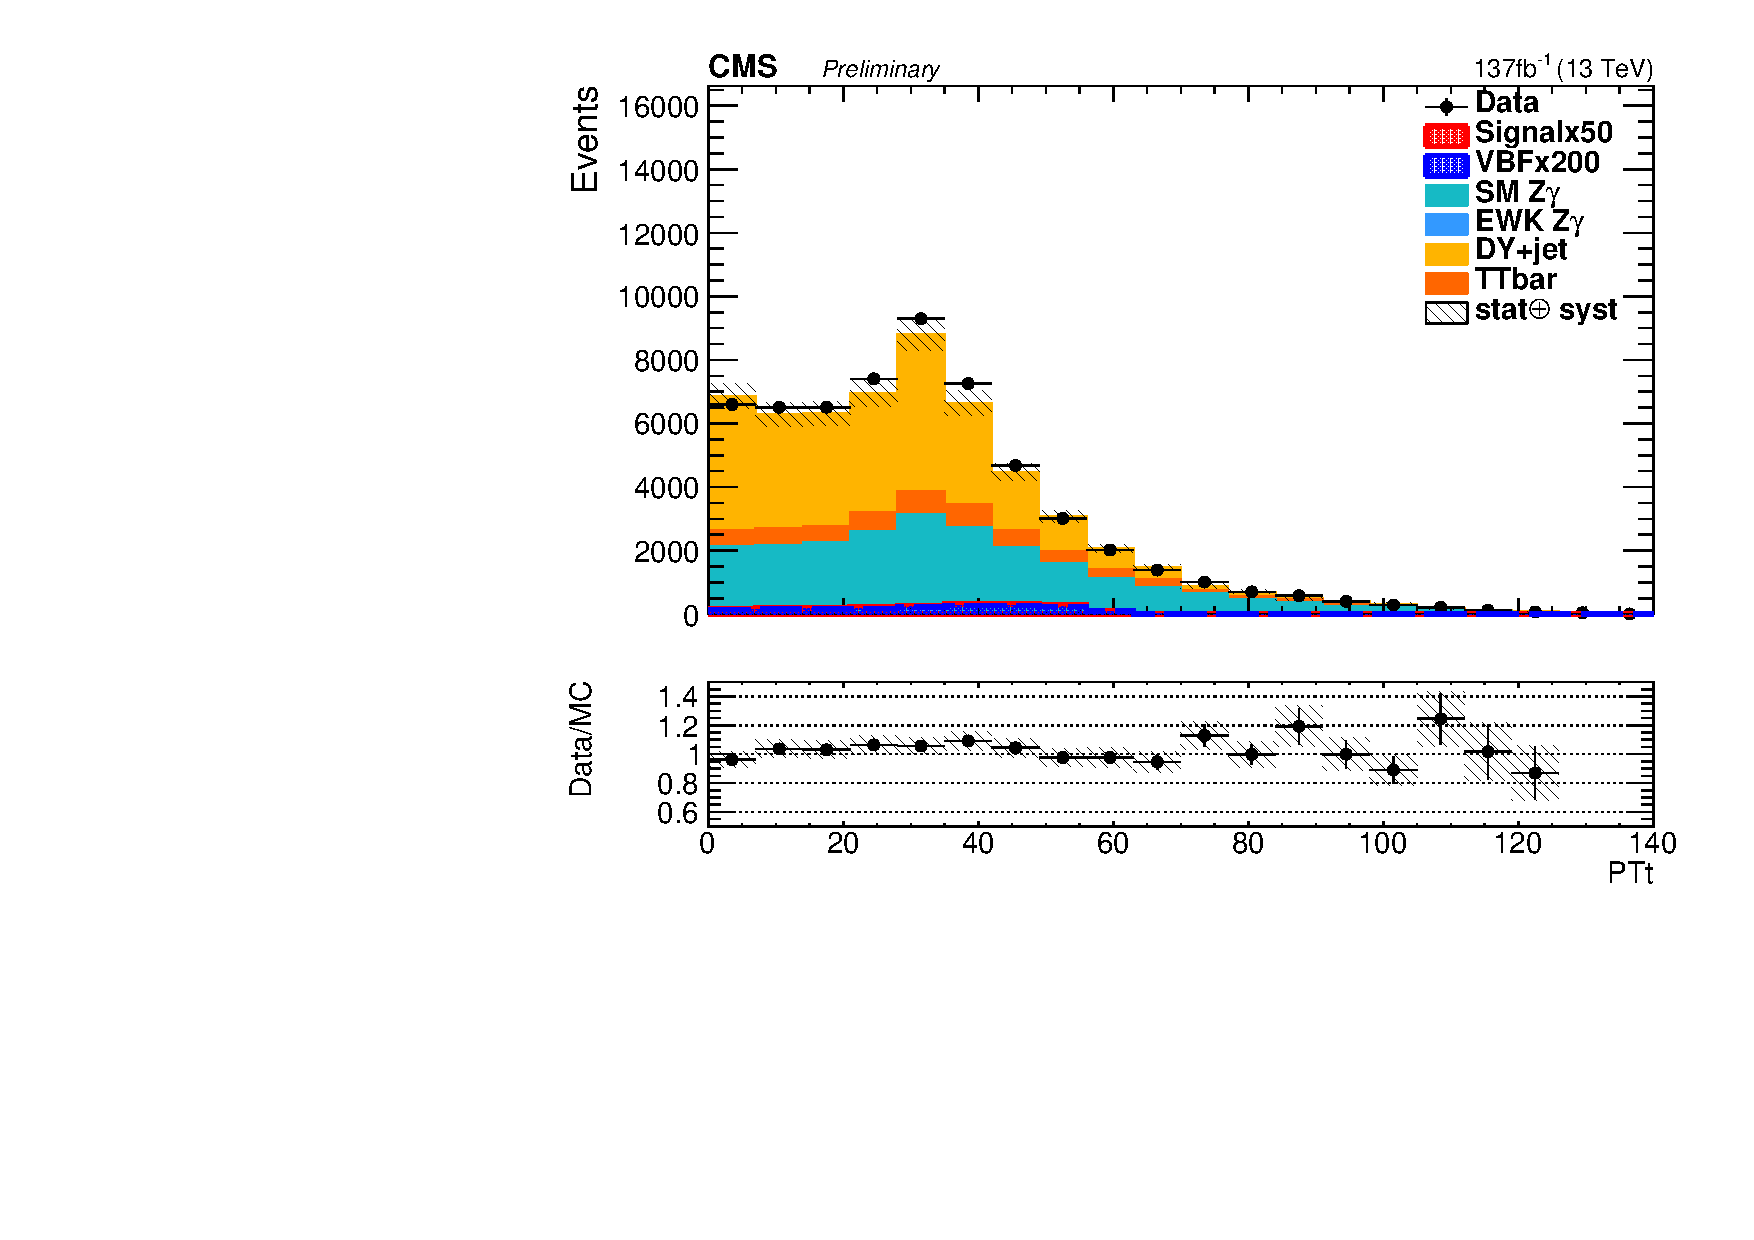
\includegraphics[width=0.3\textwidth]{fig/MVA/sc_all_VBF_PTt_valid_ptwei_cat0.pdf}
		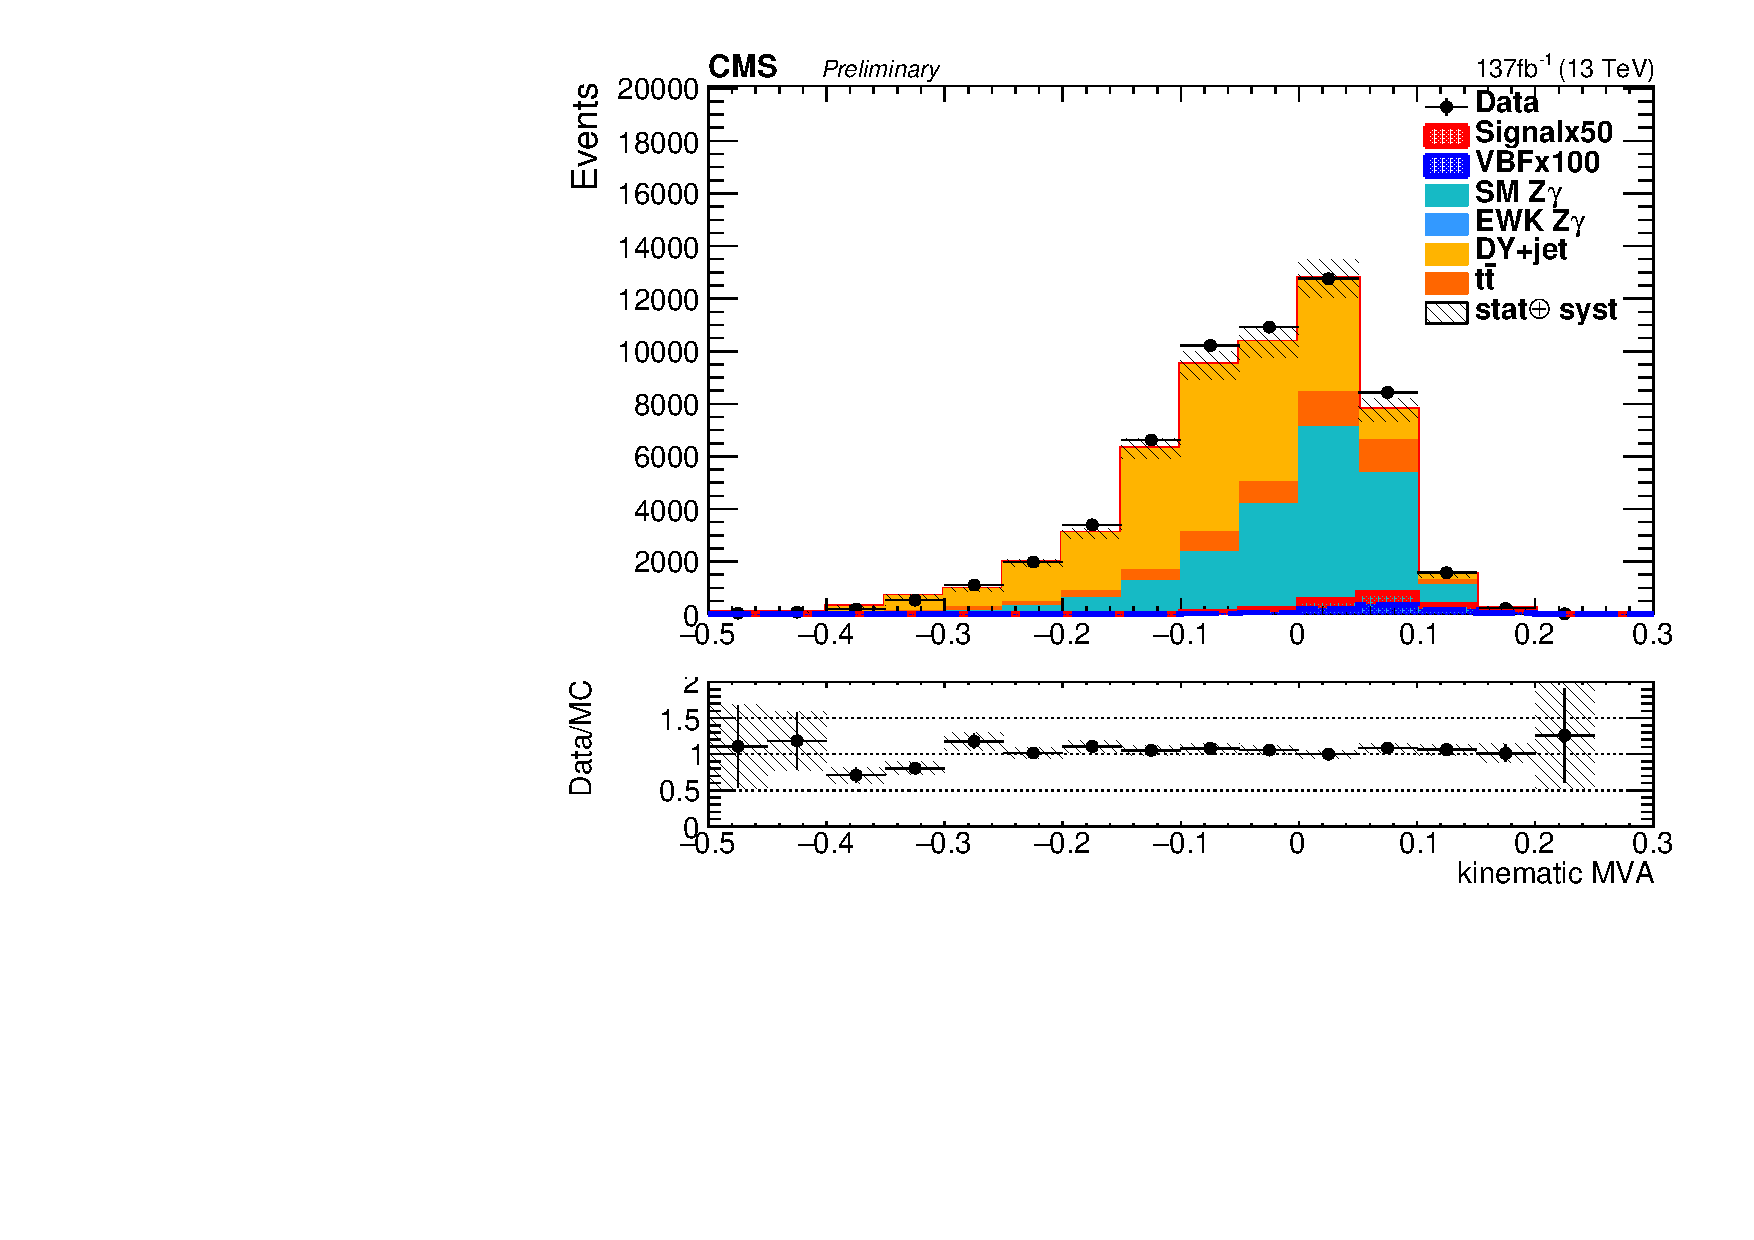
\includegraphics[width=0.3\textwidth]{fig/MVA/sc_all_VBF_kinMVA_valid_ptwei_VBF_cat0.pdf}
		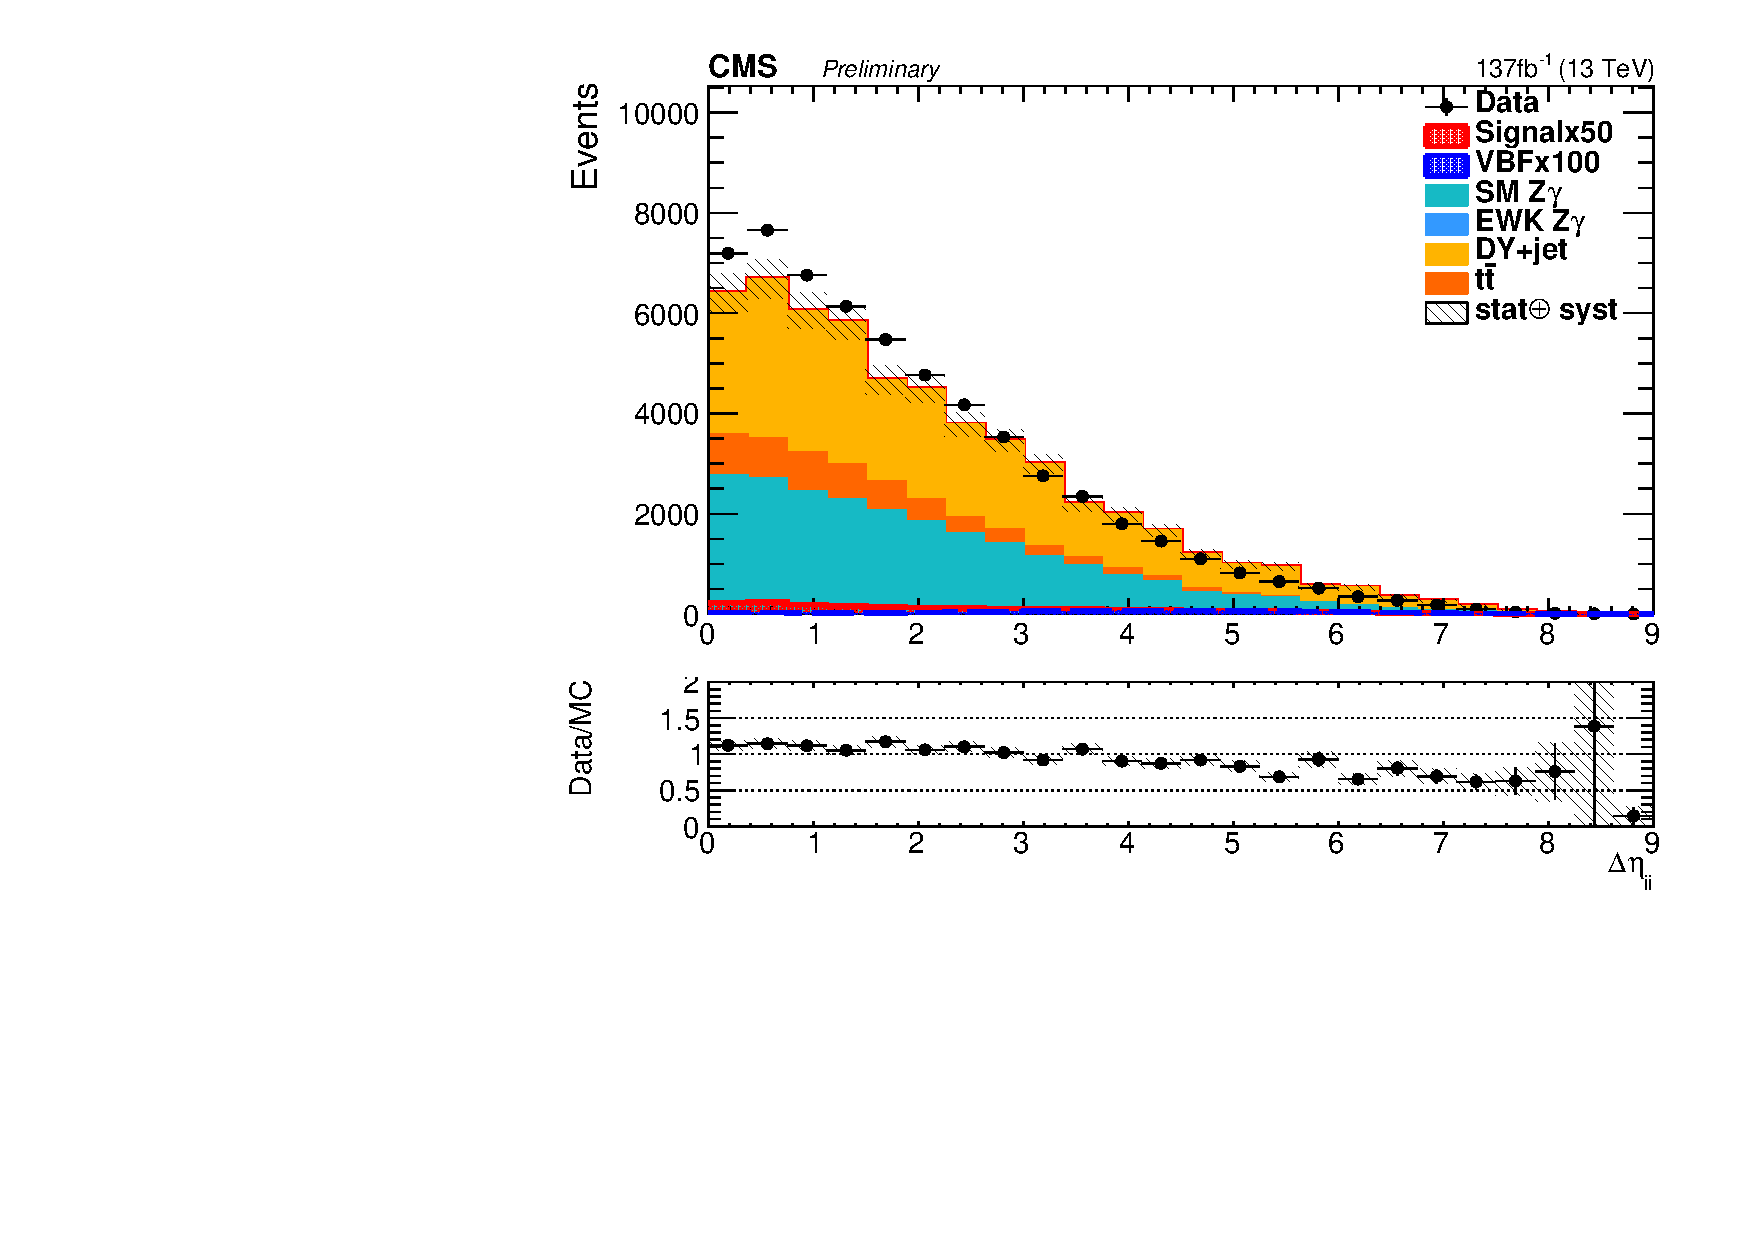
\includegraphics[width=0.3\textwidth]{fig/MVA/sc_all_VBF_dEtajj_valid_ptwei_VBF_cat0.pdf}
		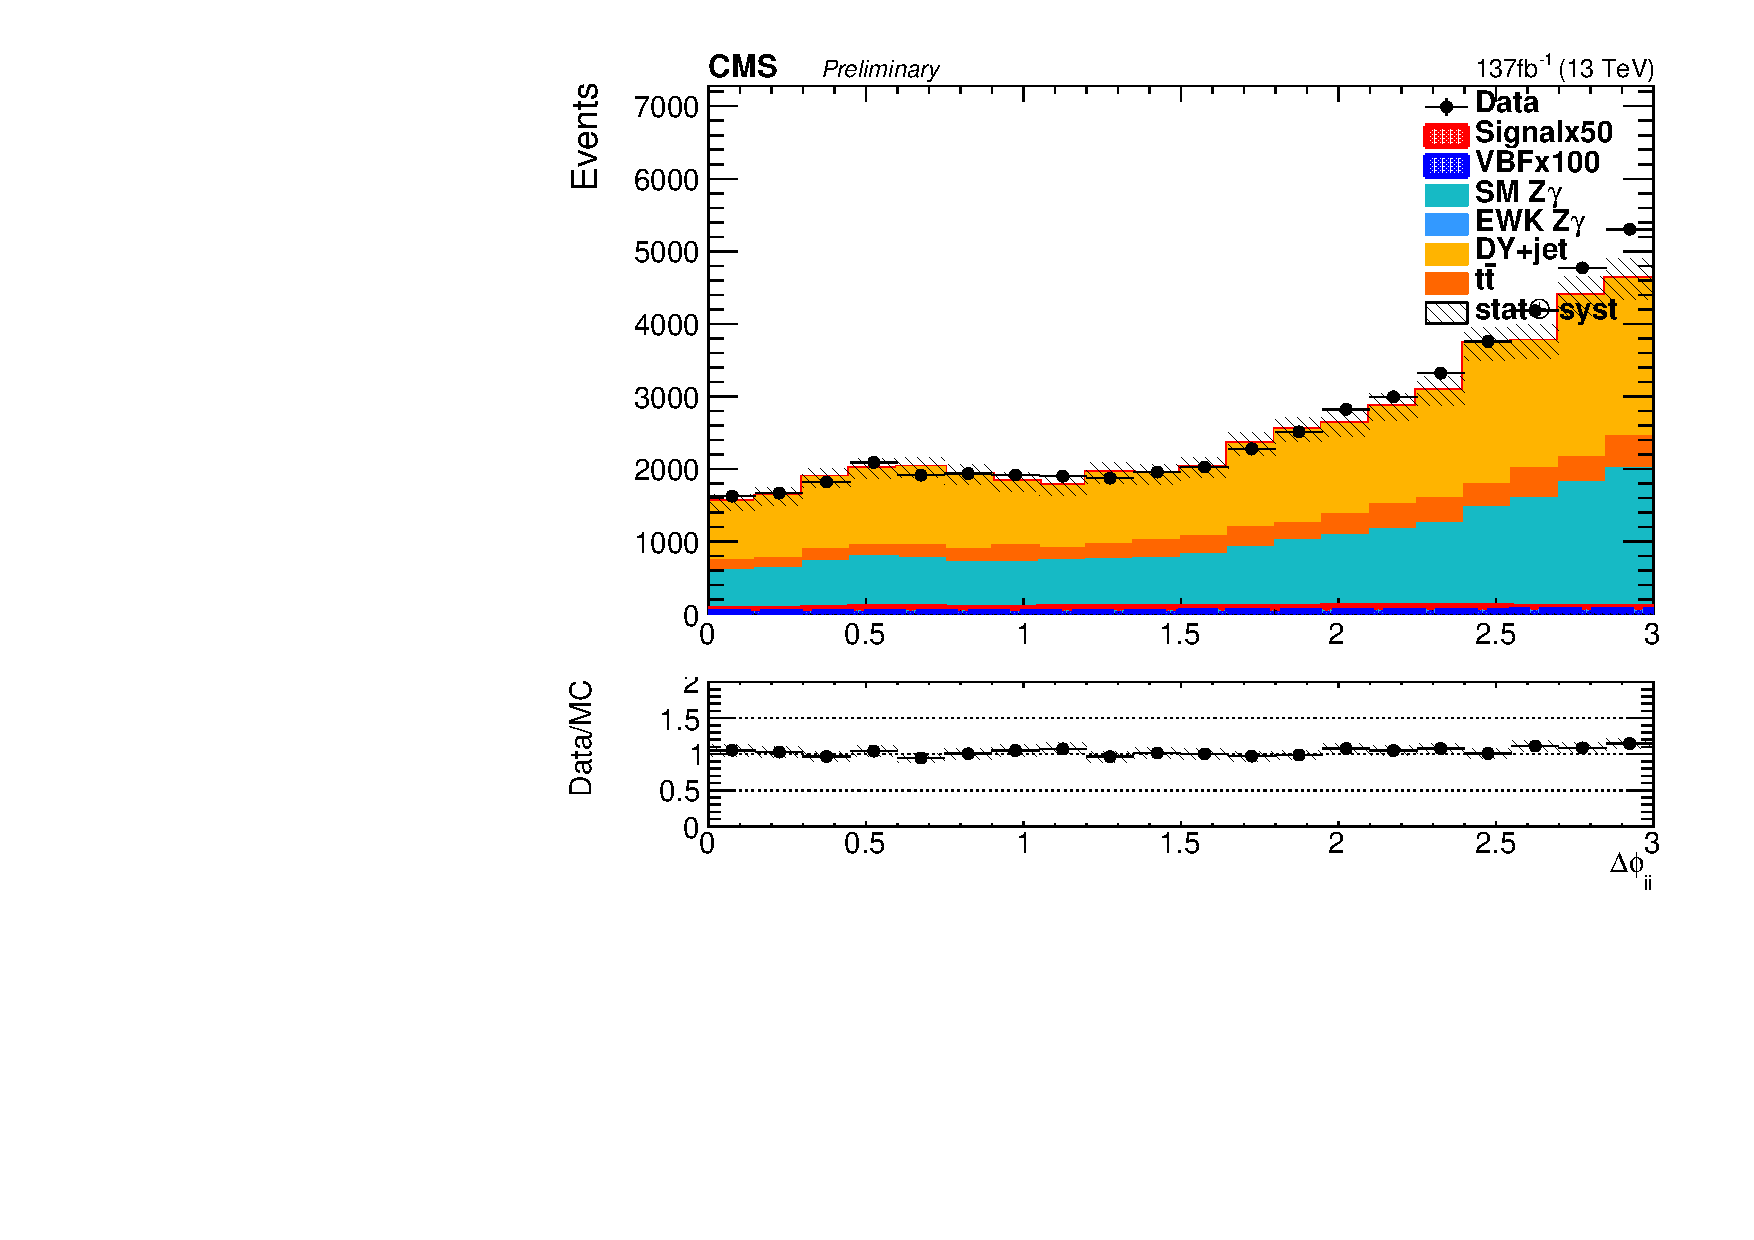
\includegraphics[width=0.3\textwidth]{fig/MVA/sc_all_VBF_dPhijj_valid_ptwei_VBF_cat0.pdf}
		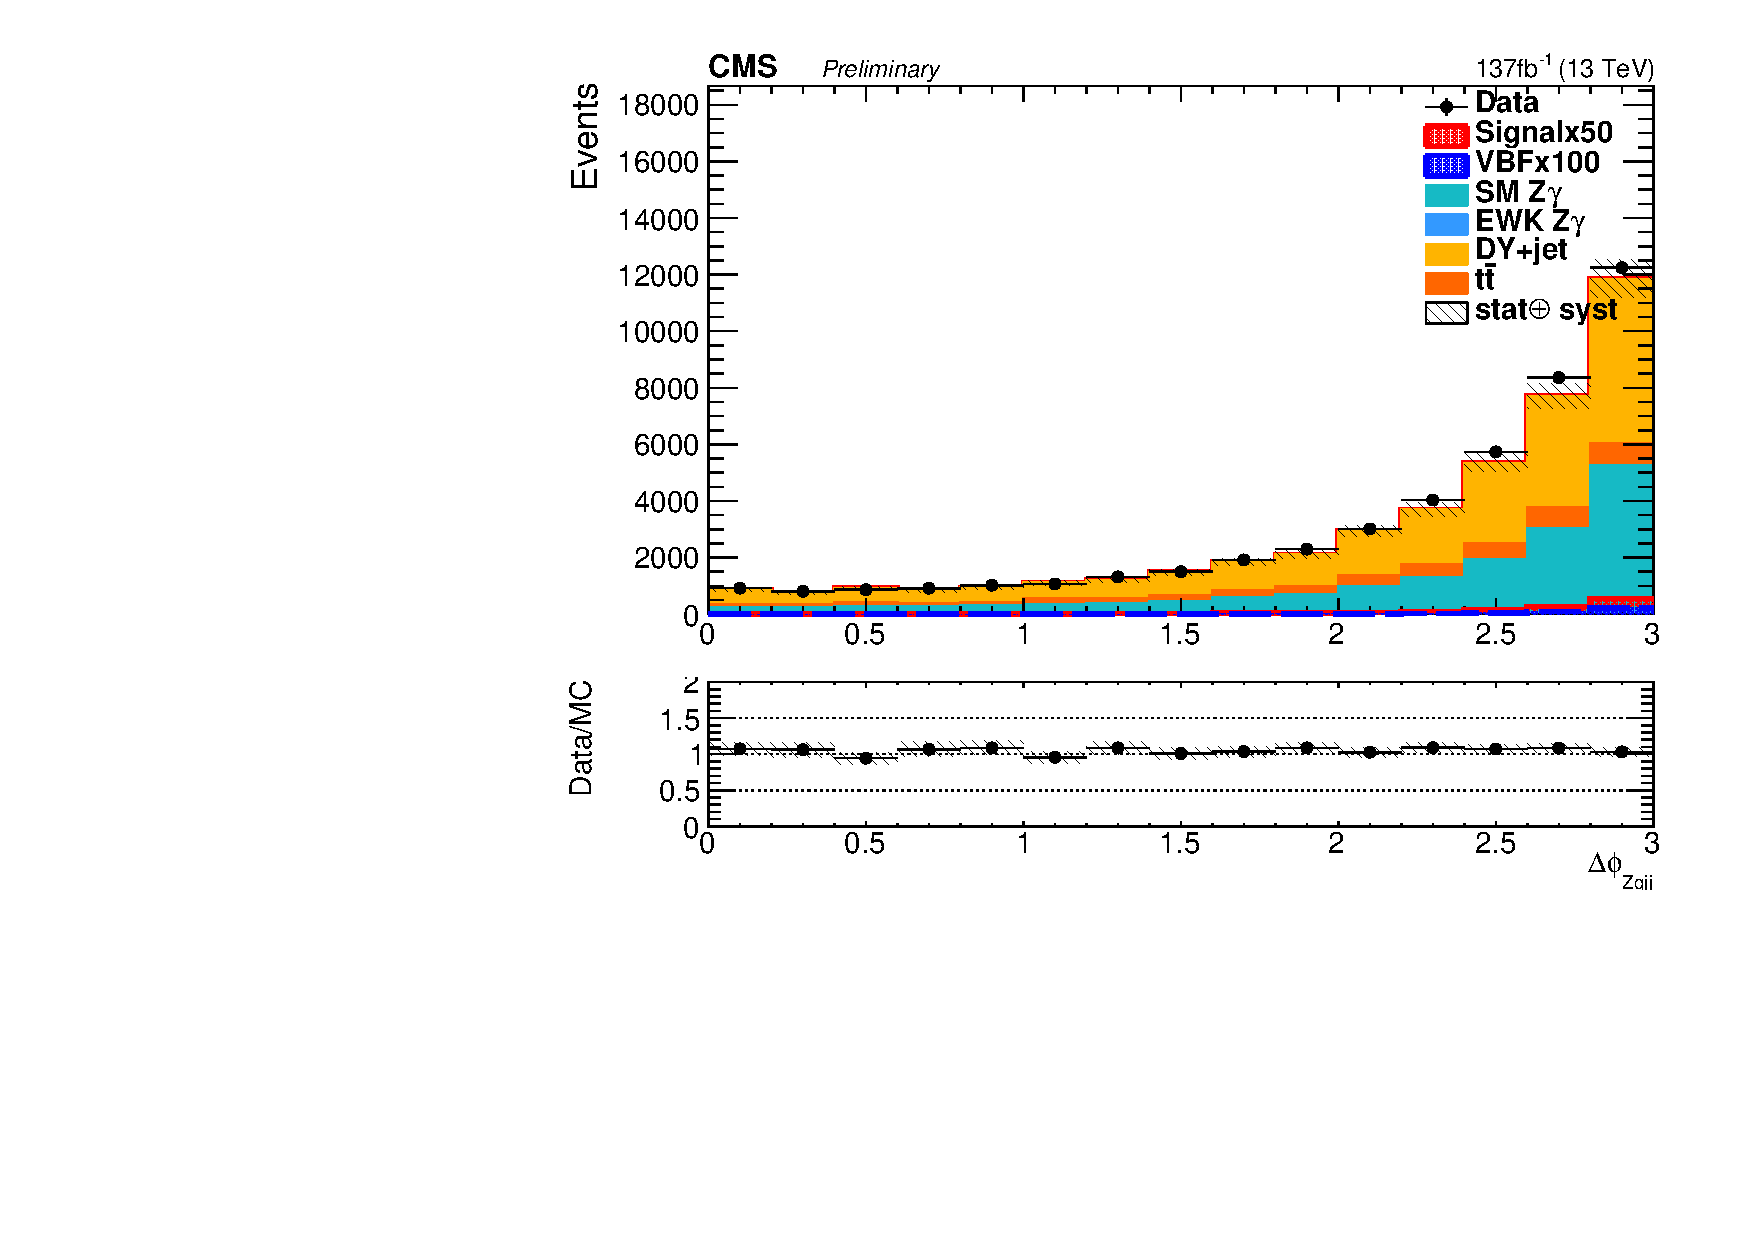
\includegraphics[width=0.3\textwidth]{fig/MVA/sc_all_VBF_dPhiZgjj_valid_ptwei_VBF_cat0.pdf}
		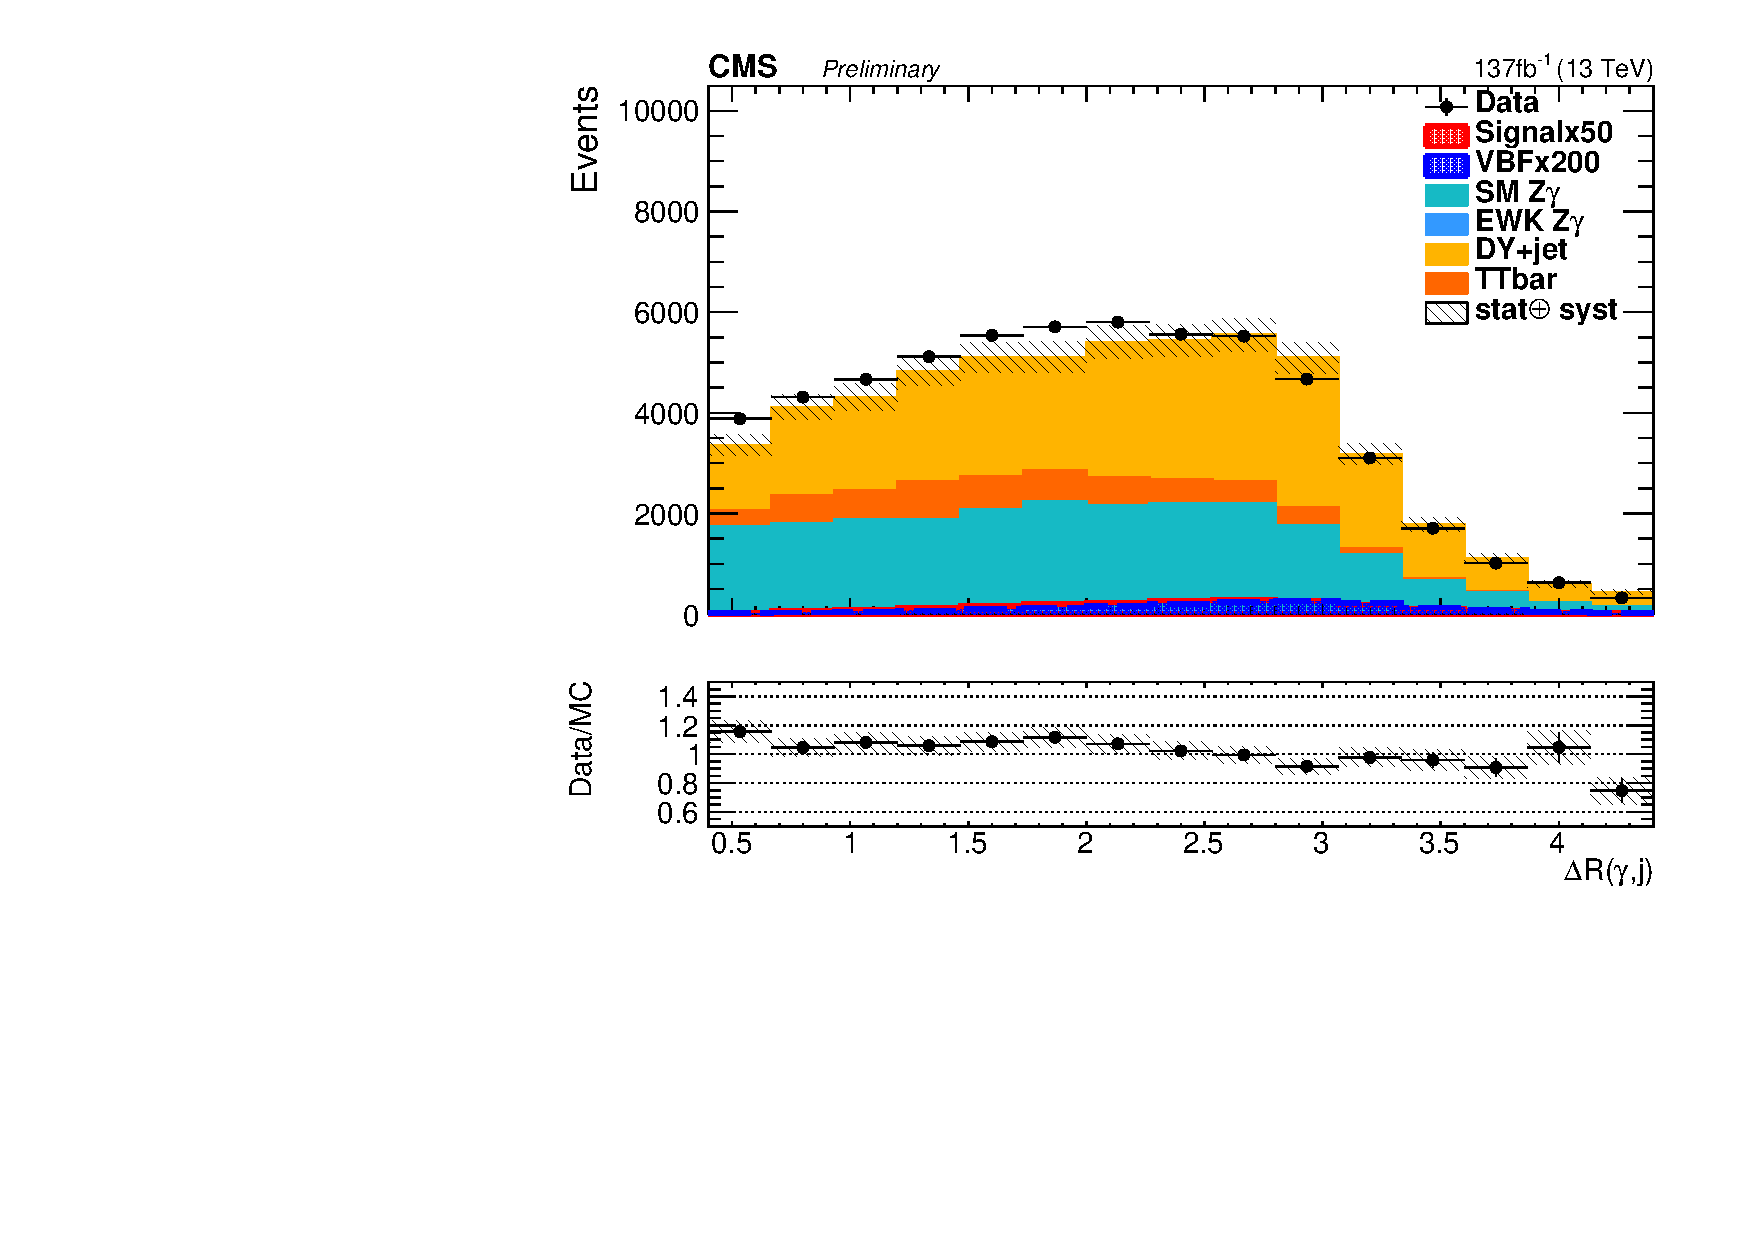
\includegraphics[width=0.3\textwidth]{fig/MVA/sc_all_VBF_dR_phojet_valid_ptwei_cat0.pdf}
		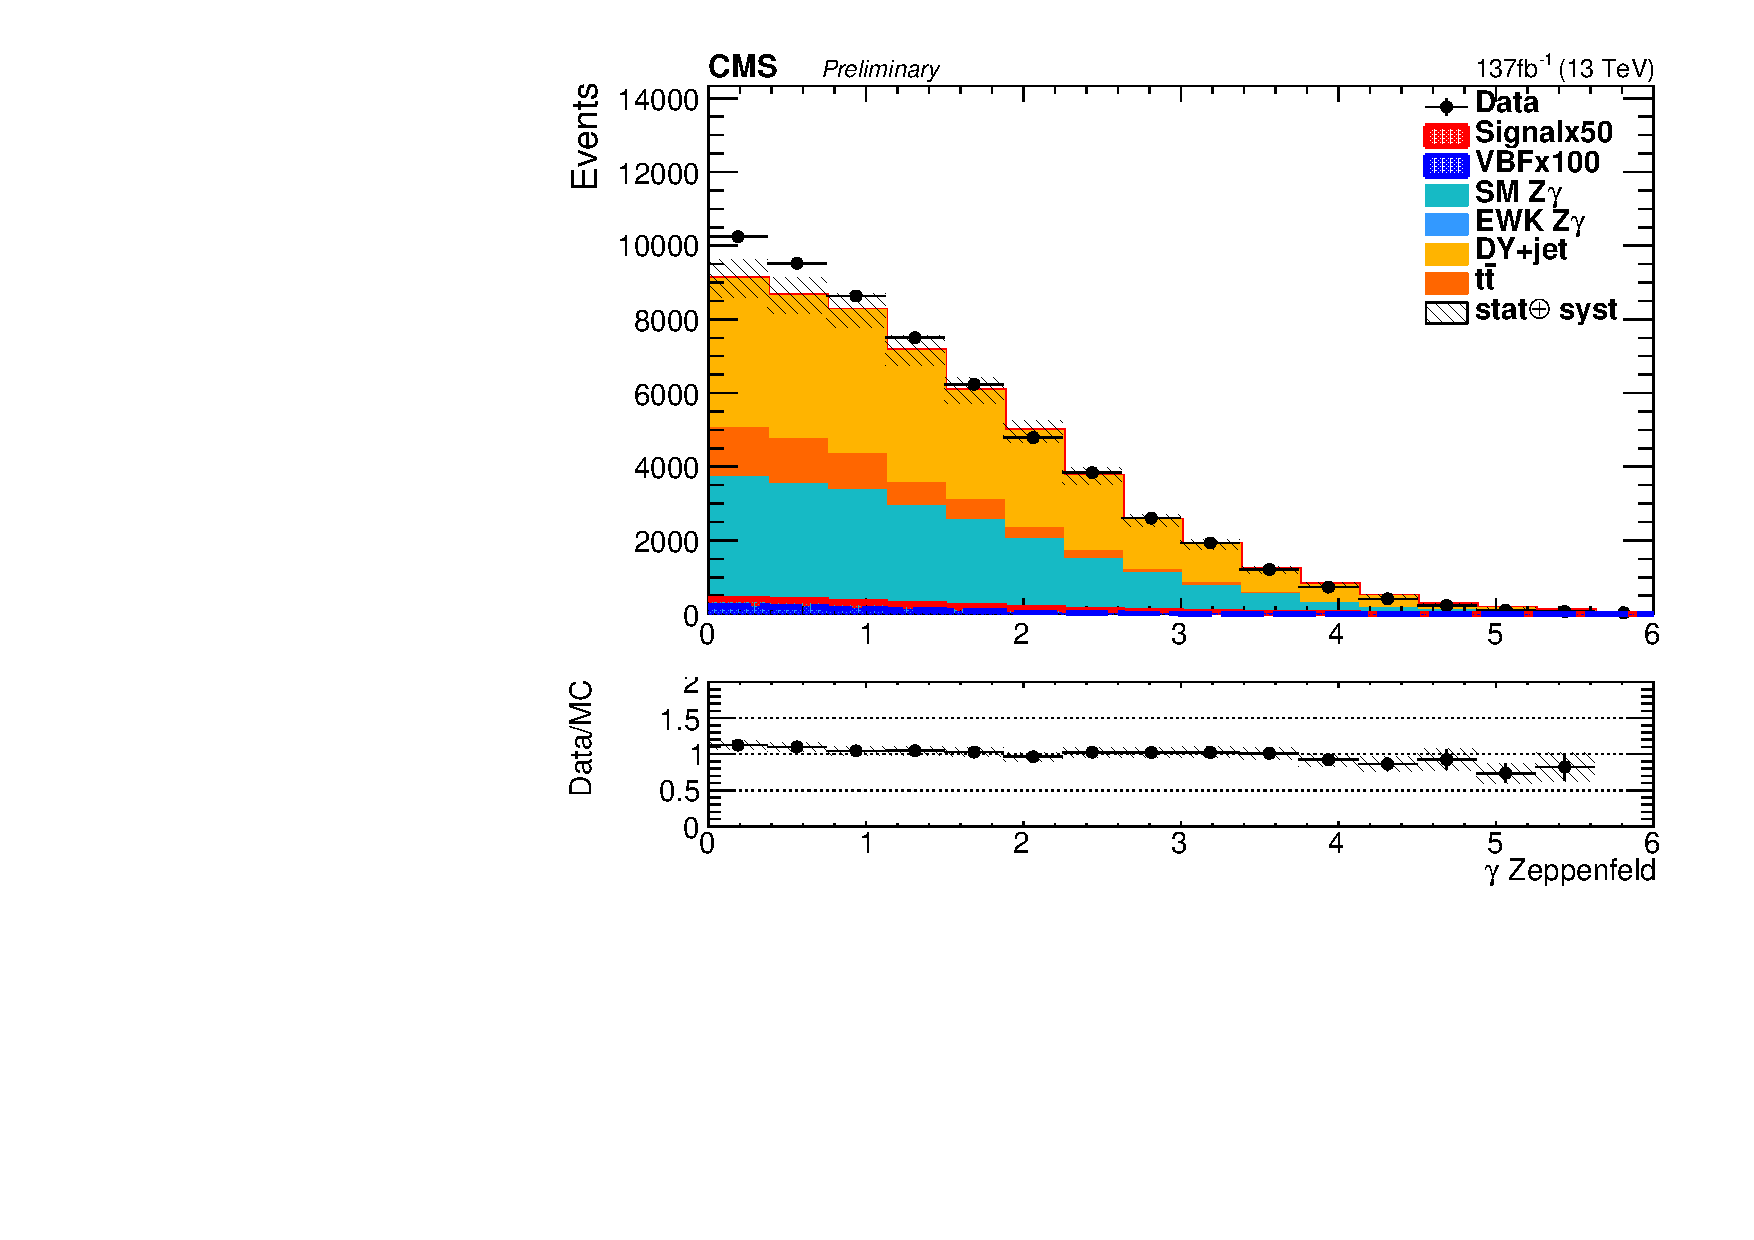
\includegraphics[width=0.3\textwidth]{fig/MVA/sc_all_VBF_Zeppen_pho_valid_ptwei_VBF_cat0.pdf}
		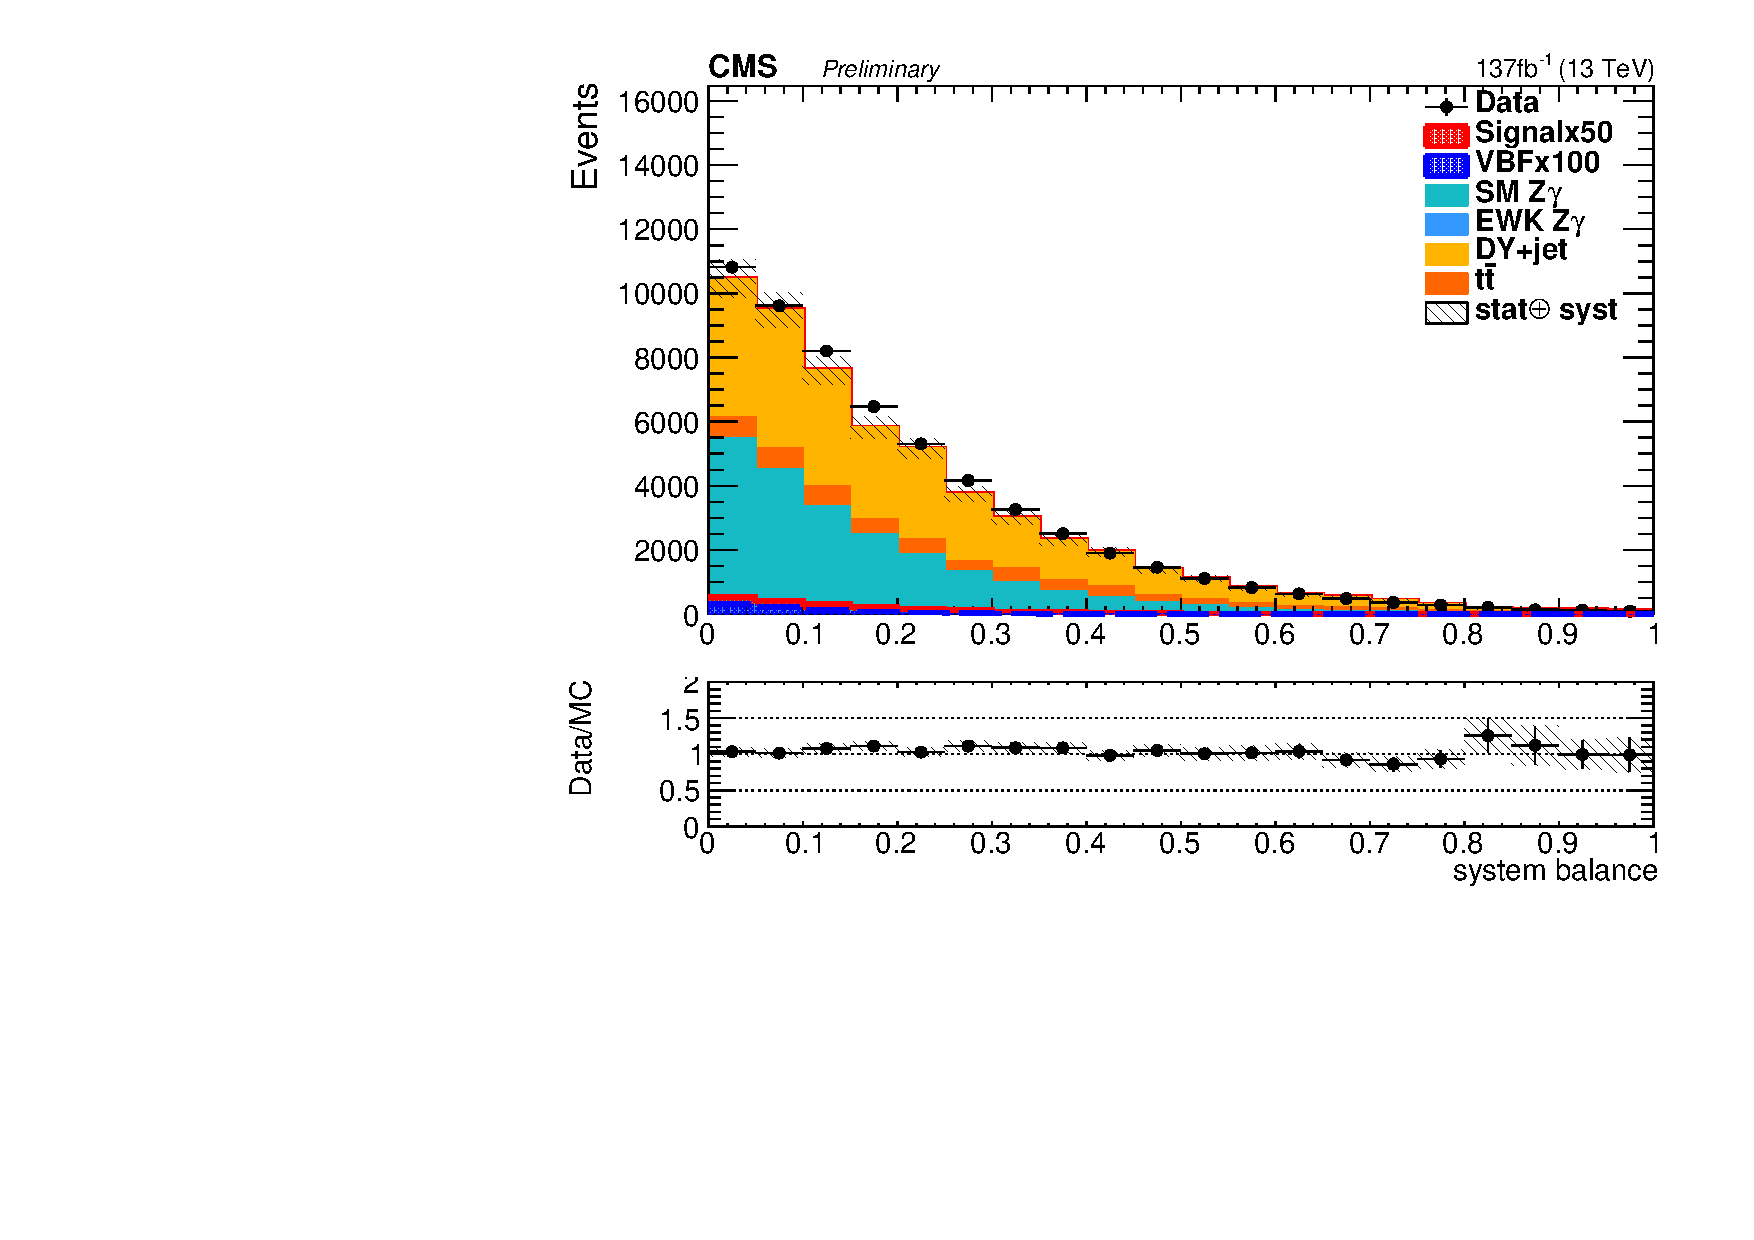
\includegraphics[width=0.3\textwidth]{fig/MVA/sc_all_VBF_sysbal_valid_ptwei_VBF_cat0.pdf}\\ 
		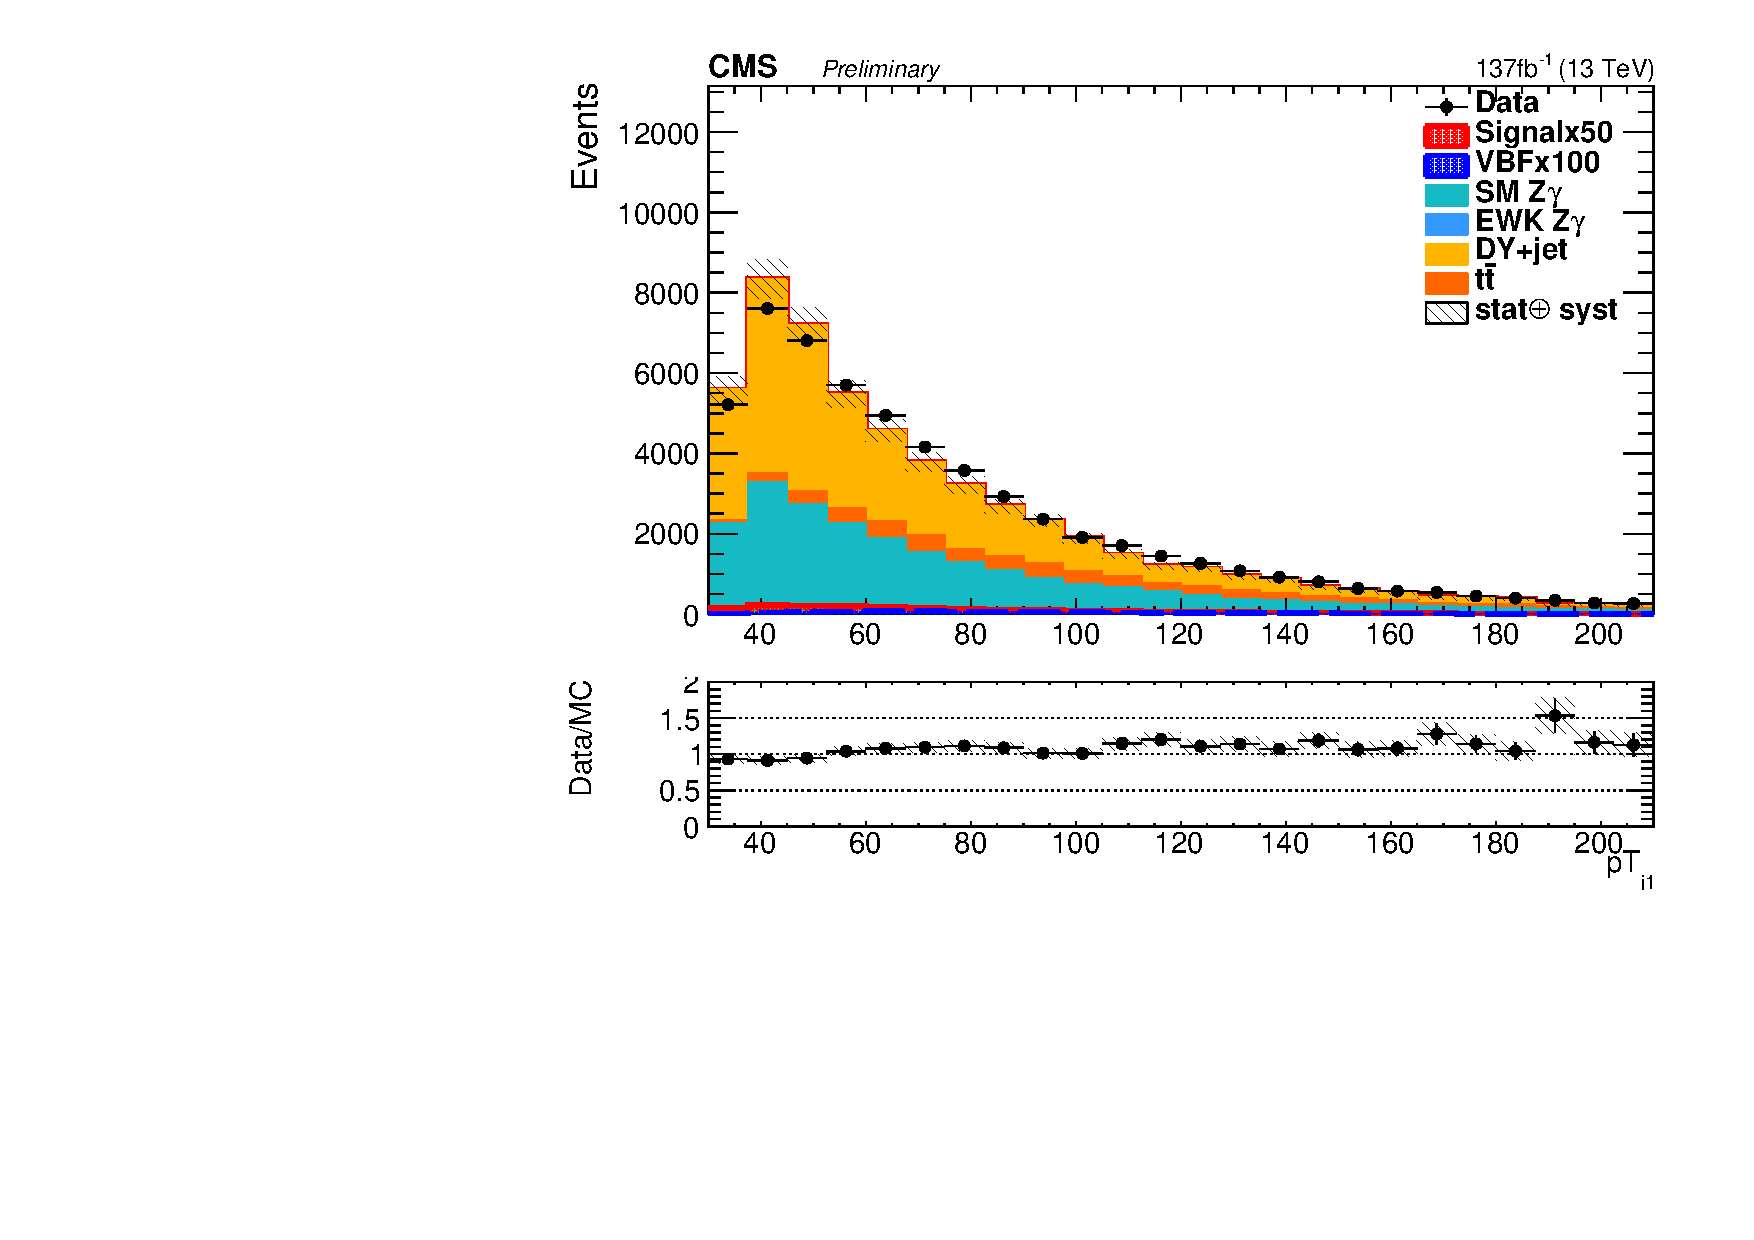
\includegraphics[width=0.3\textwidth]{fig/MVA/sc_all_VBF_VBFPt1_valid_ptwei_VBF_cat0.pdf}
		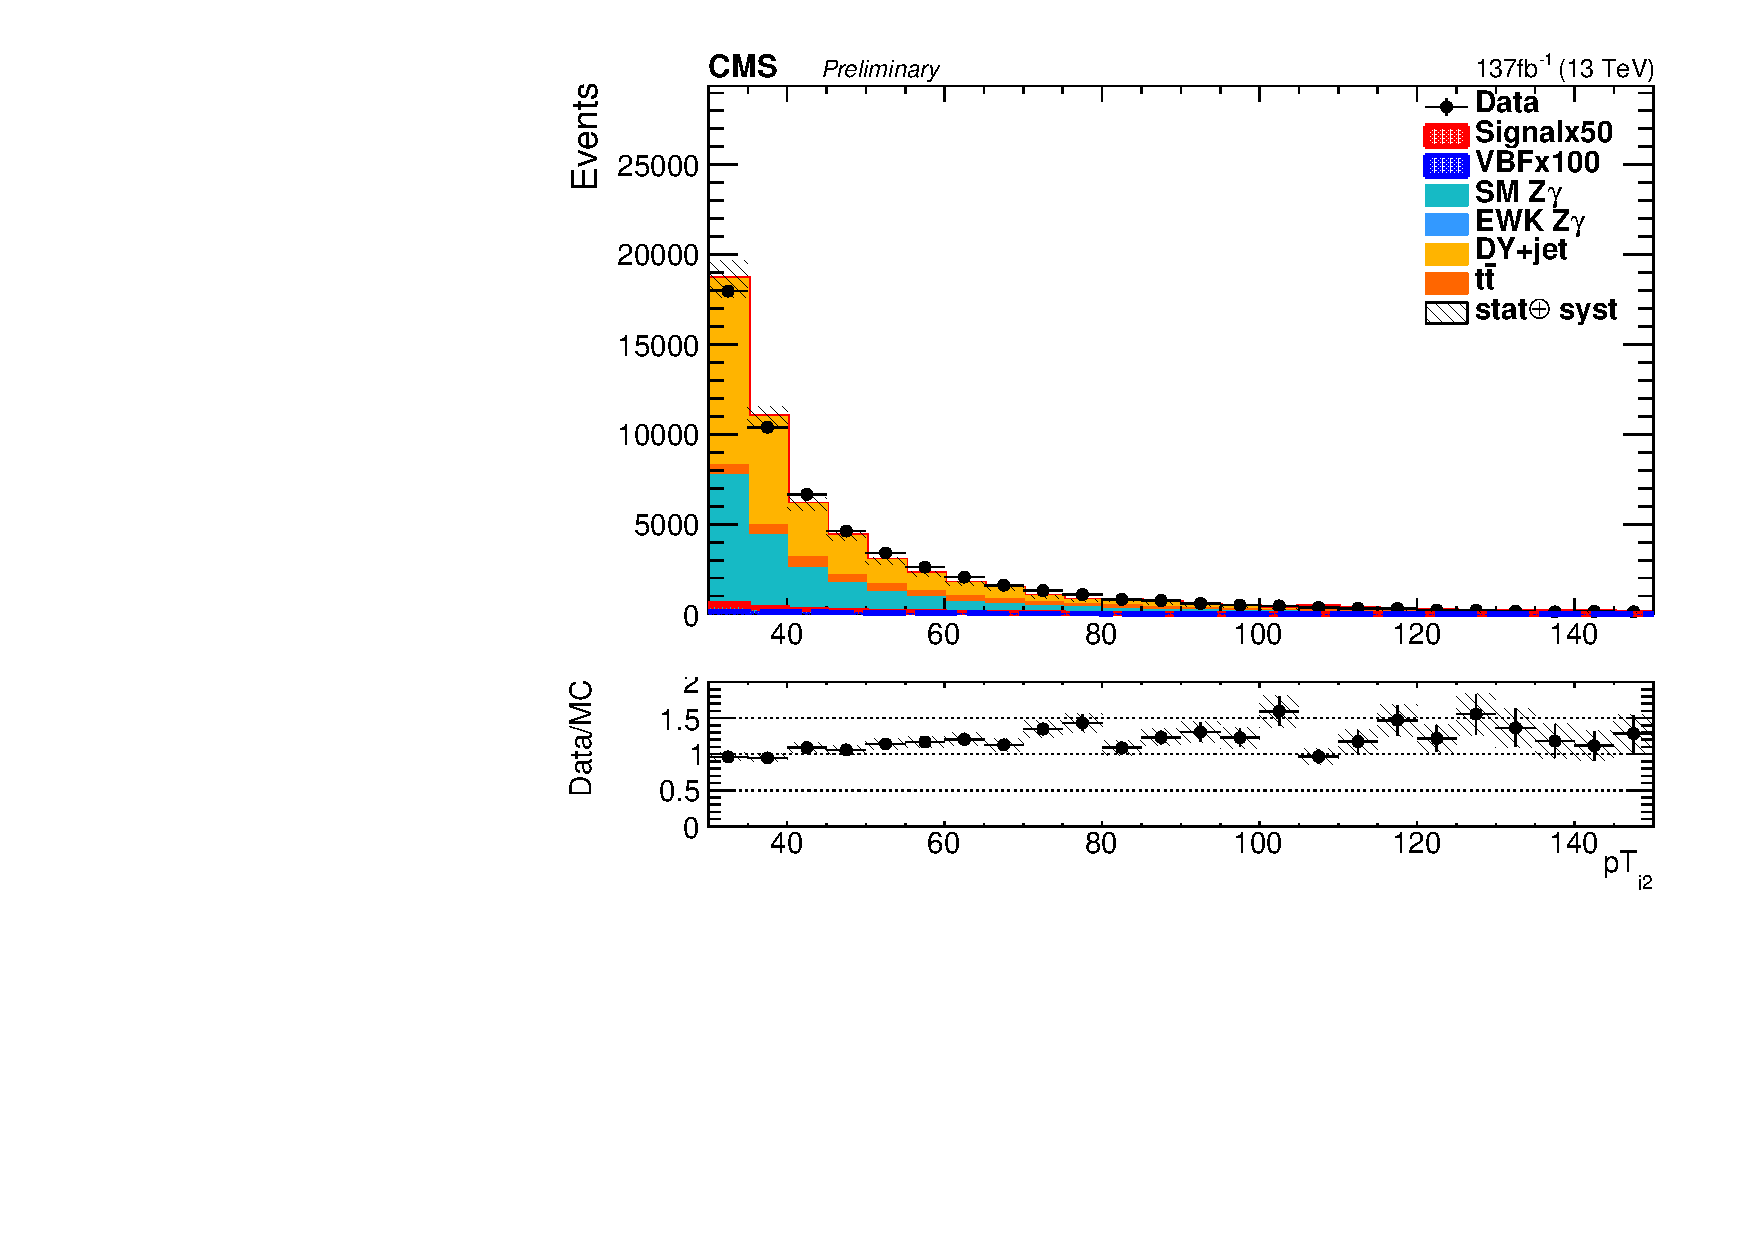
\includegraphics[width=0.3\textwidth]{fig/MVA/sc_all_VBF_VBFPt2_valid_ptwei_VBF_cat0.pdf}
		\end{center}
	\caption{Comparison of data and simulation for the VBF BDT training features. The plotted distributions include data and simulated samples from the combination of the three 
	data-taking years in both the electron and muon channels.}
	\label{fig:VBF_valid}
\end{figure}

\subsection{Training Results}
The output VBF BDT shapes for signal and background are shown in Fig.~\ref{fig:vbf_overtrain}. No overtraining is observed, 
as evidenced by the similarity between training and test distributions. The importance of each training feature for the discrimination power of
the final VBF BDT discriminant is given in Table~\ref{tab:vbf_importance}. We see that the most important feature is the $\Delta \eta$ between the jets, followed 
by the kinematic BDT score and quantities relating the dijet system to the $\PZ\gamma$ system.

\begin{figure}[tb]
	\begin{center}
		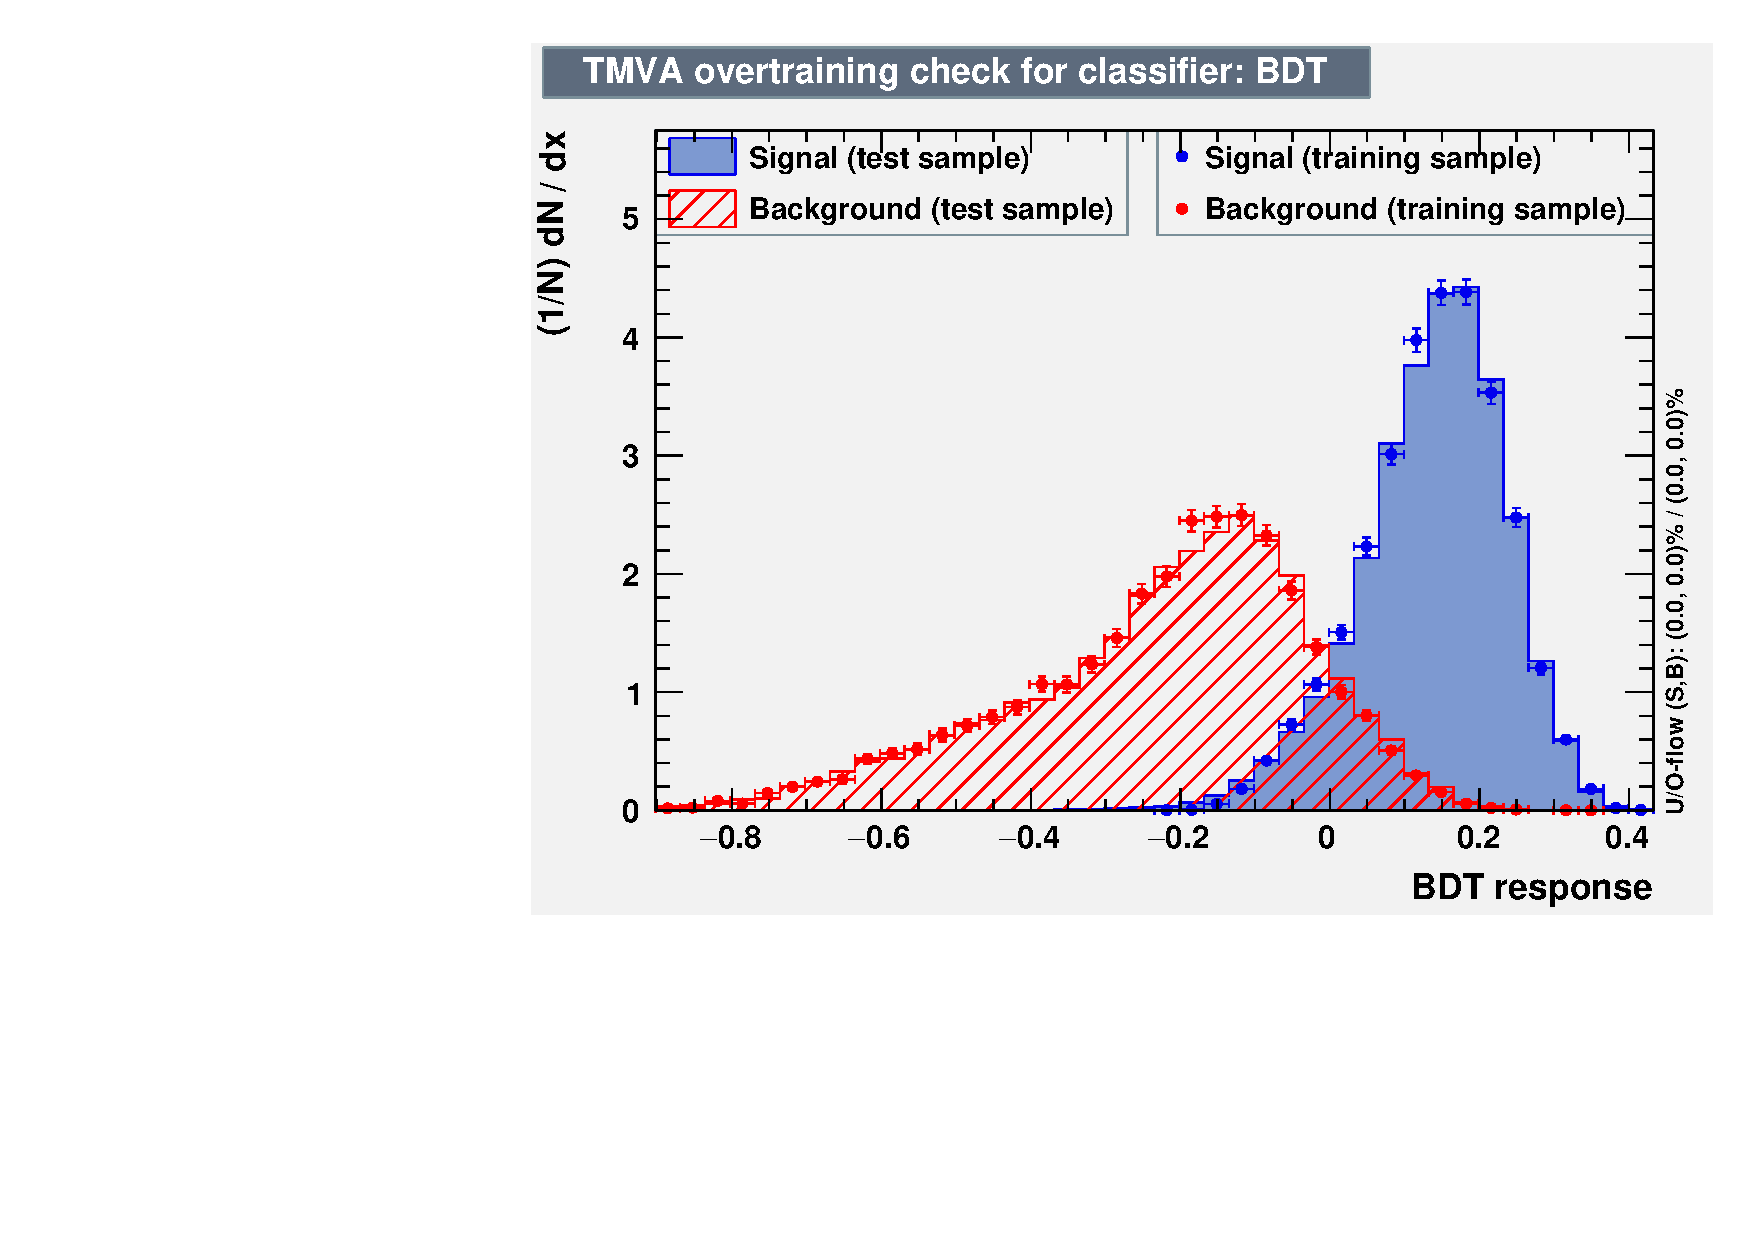
\includegraphics[width=0.65\textwidth]{fig/MVA/overtrain_BDT_VBF_WP90.pdf}
	\end{center}
	\caption{Shapes of the VBF BDT distributions for signal and background for both training and test sets. No BDT overtraining is observed.}\label{fig:vbf_overtrain}
	\label{fig:vbf_overtrain}
\end{figure}

\begin{table}[tb]
	\centering
	\begin{tabular}{|cc|}
		\hline
		      Variable       						& Variable Importance (\%) \\ \hline
		$|\Delta\eta(j_1, j_2)|$ 									& 15.9   \\
		   kinematic BDT score  						 			 	& 12.3 \\
		   $|\Delta\phi(\PZ\gamma, j_1j_2)|$  								& 11.7 \\
		 $|\sum_{\PZ\gamma j_1 j_2}\vec{\pt}/\sum_{\PZ\gamma j_1 j_2}\pt|$     	& 11.4 \\
		 $p_T^t$  		   							& 10.7  \\
		$|\Delta\phi(j_1, j_2)|$ 									& 10.4 \\
		       $|\eta_\gamma-\frac{\eta_{j1}+\eta_{j2}}{2}|$   					& 8.6 \\
		       $\pt^{j2}$  									& 7.8 \\
		      $\pt^{j1}$  									& 6.2 \\
		     $\Delta R(\gamma,j)$    								& 5.0 \\ \hline
	\end{tabular}
	\caption{Importance of the VBF BDT training features.} 
\label{tab:vbf_importance}
\end{table}

\section{Categorization Procedure}

The procedure used for event categorization is described below. 

\begin{enumerate}
  \item Events with at least one additional electron (muon) with $\pt>7$ (5)\GeV are assigned to 
	  the lepton-tagged category.
  \item Events not assigned to the lepton-tagged category, but which contain two jets satisfying the 
	  selection requirements described in Chapter~\ref{sec:selection}, are classified 
	  as dijet events, indicative of possible VBF production. 
	  The subdivision of dijet events into a set of three dijet categories using the VBF BDT is described below.
  \item Events not assigned to the lepton-tagged or dijet categories are classified as untagged events.
	The subdivision of untagged events into a set of four untagged categories using the kinematic BDT is described below.
\end{enumerate}

\begin{figure}[tbp!]
\centering
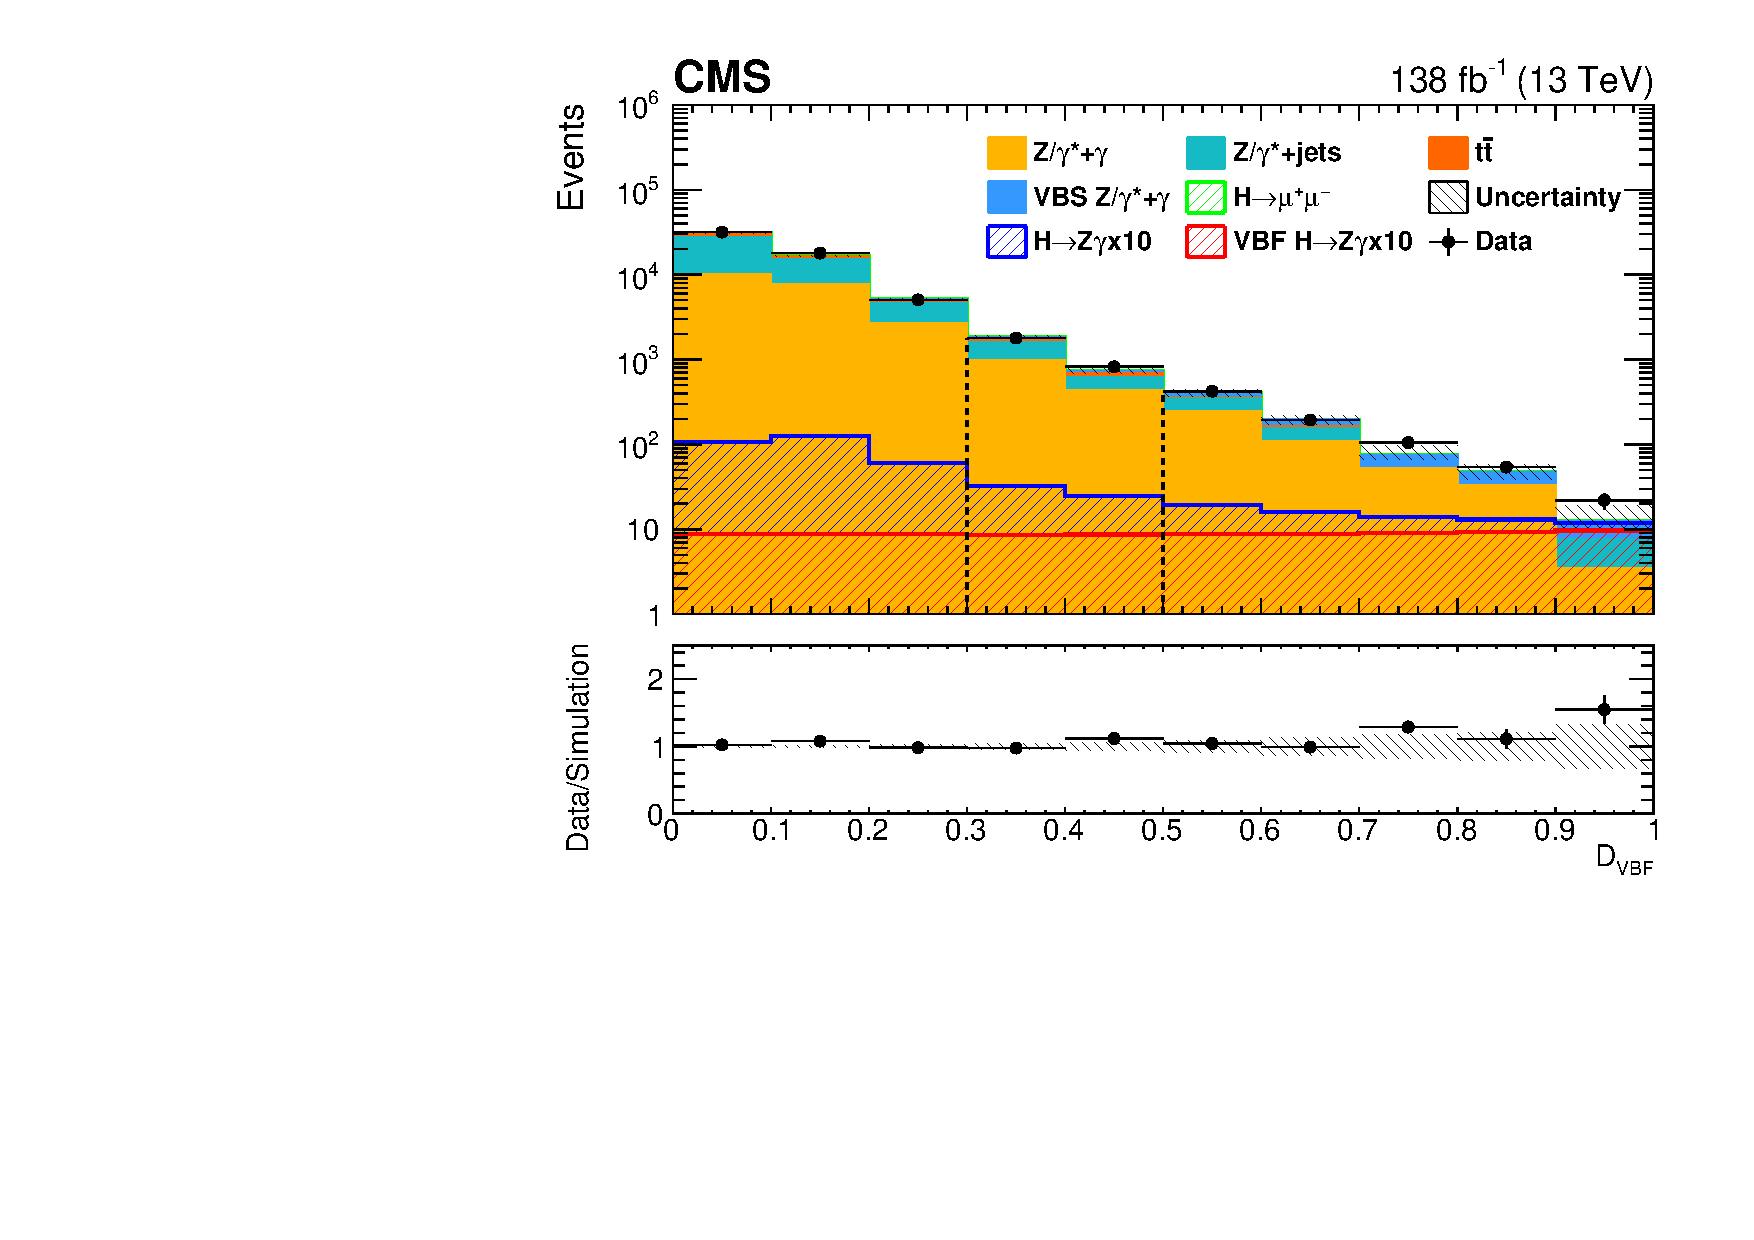
\includegraphics[width=0.47\textwidth]{fig/cat/Figure_002-a.pdf}
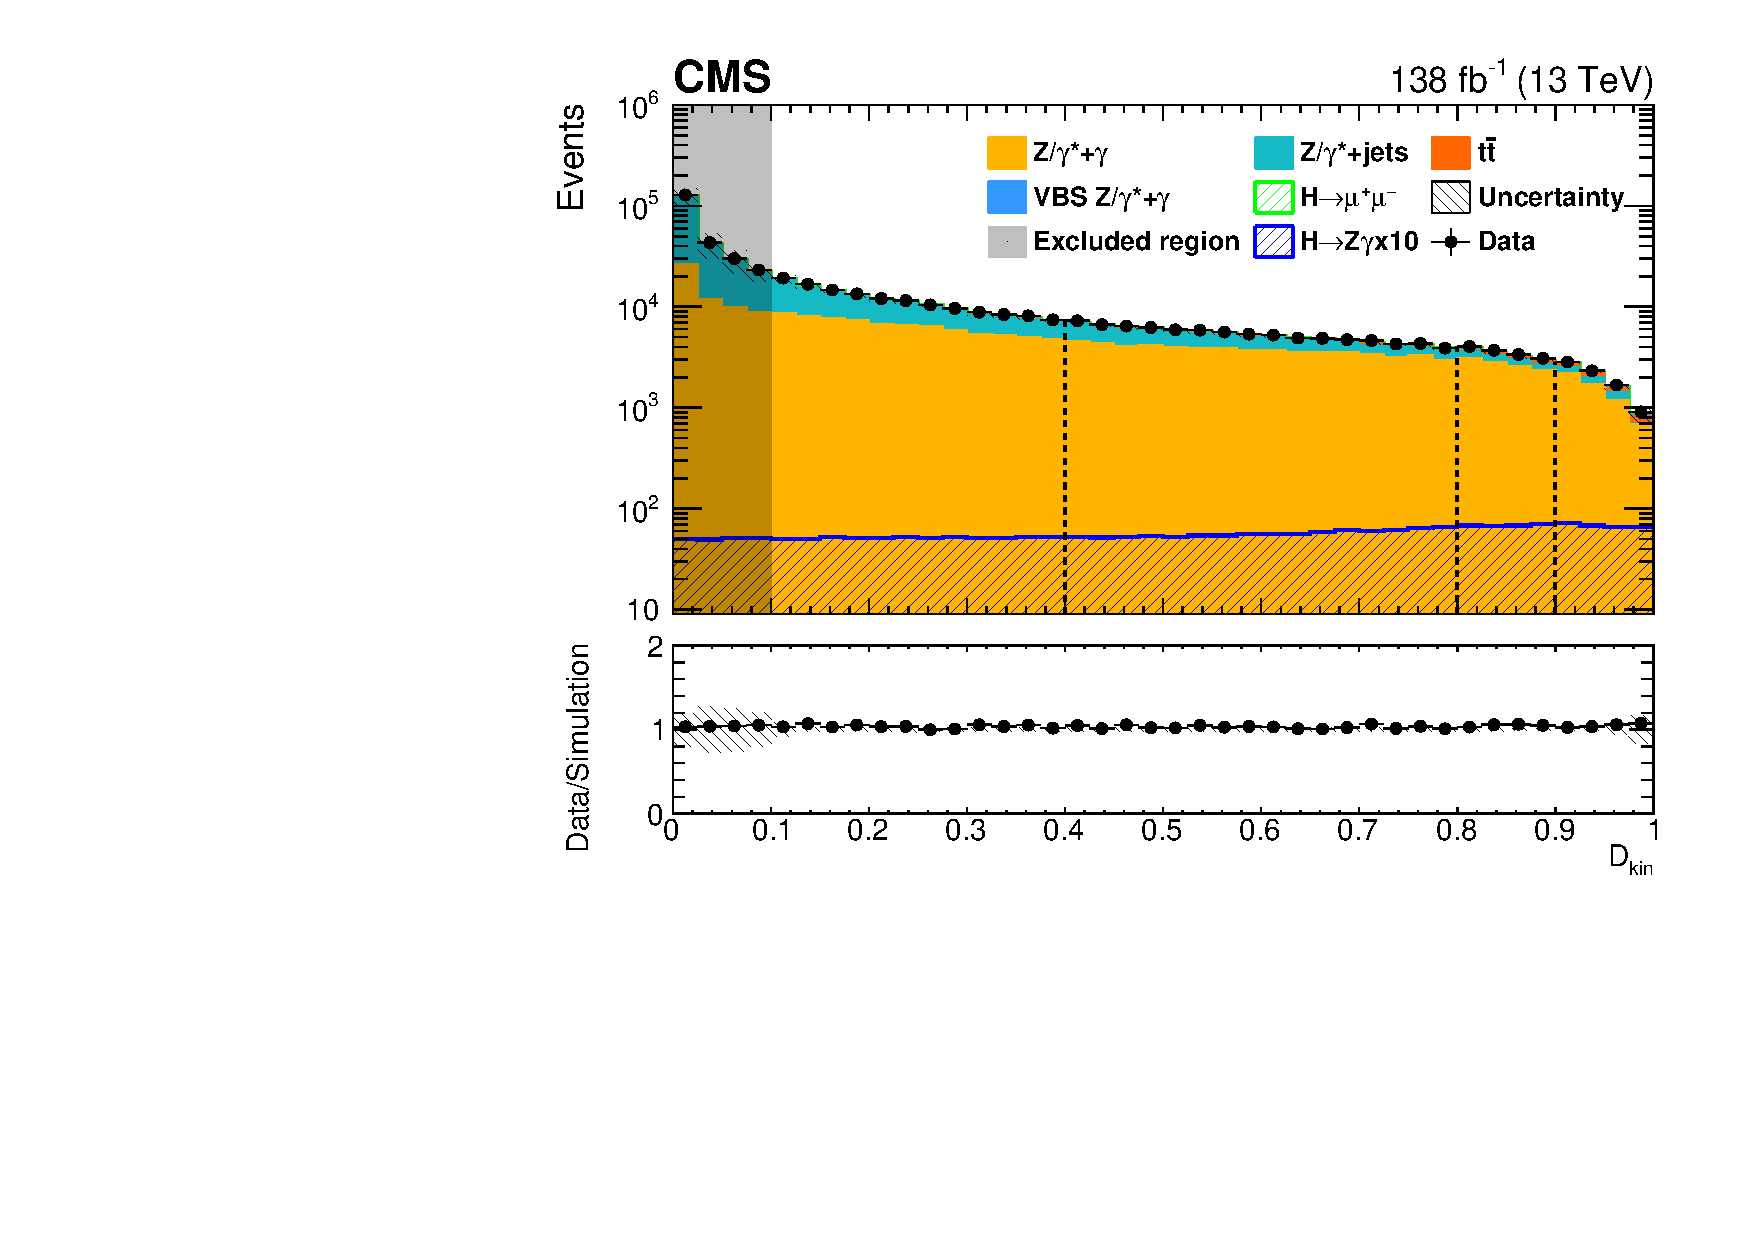
\includegraphics[width=0.47\textwidth]{fig/cat/Figure_002-b.pdf}
 \caption{The $\DVBF$ (left) and $\Dkin$ (right) distributions for signal, simulated background, and data. 
	  The $\DVBF$ distribution includes
	  only dijet-tagged events, and the $\Dkin$ distribution includes only untagged events. The sum of contributions from all signal production mechanisms is shown by the blue line, while the contribution from only the VBF mechanism is shown by the red line. The uncertainty band incorporates all statistical and systematic uncertainties in the expected background. The dashed lines indicate the boundaries for the dijet and untagged categories. The gray shaded region in the $\Dkin$ distribution is excluded from the analysis.\label{fig:BDT}}
\end{figure}

Distributions of the transformed VBF BDT score ($\DVBF$) and transformed kinematic BDT score ($\Dkin$) are shown in Fig.~\ref{fig:BDT}.
The subdivision of dijet and untagged events into categories is based on these distributions.
Category boundaries are defined as mutually exclusive regions of $\DVBF$ and $\Dkin$. 
The locations of the boundaries defining the categories are optimized by iterating over all possible combinations of boundaries using $\sum_{i=1}^{n} {S_i}^2/B_i$
as a figure-of-merit. The variables $S_i$ and $B_i$
represent the number of expected signal and background events in the ${i}^{th}$  
category, and $n$ is the total number of categories. 
We consider categories with boundaries corresponding to signal efficiencies  
between 0 and 100\% in 10\% increments.
This optimization procedure results in three dijet categories and four untagged categories.
The lowest $\Dkin$ boundary corresponds to the 10\% point in integrated signal efficiency, 
and events below the 10\% point are excluded from the analysis to preserve the stability of the background model.

The full categorization and optimization procedure results in the following eight mutually exclusive categories: 
one lepton-tagged category, three dijet categories, and four untagged categories. 
The category definitions are summarized in Table~\ref{tab:category}.
\begin{table}[!tb]
    \centering   
    \caption{Summary of the category definitions. The lepton-tagged category requires at least one additional electron or muon. Dijet categories are defined by regions of $\DVBF$ 
	  and untagged categories are defined by regions of $\Dkin$.}
  \begin{tabular}{c@{\hskip 0.3in}ccc@{\hskip 0.3in}cccc}
    \hline
                 Lepton   & Dijet 1 & Dijet 2 & Dijet 3& Untagged 1 & Untagged 2 & Untagged 3 & Untagged 4 \\\hline
		  \multirow{2}{*}{$\geq$ 1 $\Pe,\mu$} &\multicolumn{3}{c}{$\DVBF$ selection}&\multicolumn{4}{c}{$\Dkin$ selection}\\
        &0.5--1.0&0.3--0.5&0.0--0.3&0.9--1.0&0.8--0.9&0.4--0.8&0.1--0.4\\
        \hline
  \end{tabular}
  \label{tab:category}
\end{table}

Table~\ref{tab:yield} lists the event categories used in the analysis, along with the expected event yields for an $m_{\PH}=\mH\GeV$ signal arising from 
$\Pg\Pg\PH$, VBF, $\mathrm{V}\PH$, and $\ttbar\PH$ production, as well as the resonant background contribution from FSR from $\PH\to\mpmm$, which is 3--8\% of the \hzg{} yield, depending on the category. Event yields from other Higgs backgrounds such as $\PH\to\tau^+\tau^-$ and $\PH\to\gamma\gamma$ are estimated to be below the 1\% level relative to the \hzg{} yield and are neglected.
The dominant contribution to the signal yield is generally from $\Pg\Pg\PH$ production, except in the lepton-tagged category, in which $\mathrm{V}\PH$ and $\ttbar\PH$ events dominate, and in the dijet 1 category, in which VBF events dominate.
The categorization procedure increases the sensitivity of the analysis by 24\% with respect to an inclusive event selection.  

  \begin{table}[tb]
    \centering   	
	  \tiny
    \caption{Yields and approximate significance ($S/\sqrt{B}$) for each category, where $S$ and $B$ are the expected number of signal and background events in the narrowest $m_{\lplm\gamma}$ interval containing 95\% of the expected signal distribution.
    Also shown is the $m_{\lplm\gamma}$ resolution, computed using the narrowest interval containing 68\% of the expected signal distribution. 
	   }
  \begin{tabular}{c@{\hskip 0.3in}ccccccccc}
    \LumiT\fbinv   & Lepton   &  & Dijet 1 & Dijet 2 & Dijet 3& Untagged 1 & Untagged 2 & Untagged 3 & Untagged 4\\\hline
  \tabincell{c}{\textbf{SM signal}\\\textbf{yield}}    &&        &           &           &           &        &        &        &       \\
  $\Pg\Pg\PH$             & 0.51   & \tabincell{c}{$\epem$\\$\mpmm$} & \tabincell{c}{1.10\\1.41}& \tabincell{c}{1.62\\2.05}& \tabincell{c}{9.44\\12.1}&\tabincell{c}{6.89\\8.52}& \tabincell{c}{7.35\\9.17}& \tabincell{c}{29.8\\38.0}&\tabincell{c}{22.5\\29.0}\\
  &        &           & &           &           &        &        &        &       \\
  VBF             & 0.09   & \tabincell{c}{$\epem$\\$\mpmm$}& \tabincell{c}{1.94\\2.40}& \tabincell{c}{0.76\\0.97}&  \tabincell{c}{1.13\\1.43}& \tabincell{c}{0.71\\0.89}& \tabincell{c}{0.35\\0.43}& \tabincell{c}{0.92\\1.18}& \tabincell{c}{0.51\\0.65}\\
  &        &           & &           &           &        &        &        &       \\
  $\mathrm{V}\PH+\ttbar\PH$& 1.84  & \tabincell{c}{$\epem$\\$\mpmm$} & \tabincell{c}{0.04\\0.05}& \tabincell{c}{0.13\\0.16}& \tabincell{c}{1.89\\2.36}& \tabincell{c}{0.31\\0.39}& \tabincell{c}{0.17\\0.21}& \tabincell{c}{0.45\\0.57}& \tabincell{c}{0.27\\0.33}\\\hline
  \tabincell{c}{\textbf{SM resonant} \\\textbf{background}}&&&&&&&&&\\
  $\PH\to\mpmm$     & 0.14& $\mpmm$&0.27 & 0.27 & 0.43& 0.62& 0.49 & 2.02& 1.78\\\hline
 
  \tabincell{c}{\textbf{Mass} \\\textbf{resolution}\\(\GeVns)} & 2.12& \tabincell{c}{$\epem$\\$\mpmm$}& \tabincell{c}{1.91\\1.52}& \tabincell{c}{2.06\\1.61}& \tabincell{c}{2.15\\1.72}& \tabincell{c}{1.80\\1.37}& \tabincell{c}{1.97\\1.42}& \tabincell{c}{2.12\\1.62}& \tabincell{c}{2.33\\1.83}\\
  \hline
  
  \textbf{Data yield}            & 1485   && 168    & 589    & 11596& 1485      & 1541      & 2559      & 17608   \\\hline
  \textbf{$S/\sqrt{B}$}    & 0.06  && 0.54  & 0.24  & 0.26& 0.45  & 0.35  & 0.53  & 0.30  \\
  
  \\
  \end{tabular}
  \label{tab:yield}
  \end{table}
